\section{Uniform correlations of two prescribed edges}\label{c6:subheading-14}
\label{u:marked-uniform}

We prove Theorem~\ref{u:two-edge-theorem}.  Keep its triangular-lattice
directions $e_1,e_2$, identical translated marks $E,E+P$, and
$P=P_1e_1+P_2e_2$ with $P_1,P_2>0$.  Thus $d=P_1+P_2$ is even,
the cylinder period is $kP$ with $k\ge2$, and $N=kd$.  The polygon
weight counts visited triangle centres.  Our goal is a bound uniform
both in the staircase direction and in the ratio $N/d$.

The two restrictions on the marked edge and displacement let us place
both marks on a monotone staircase of period $P$.  The parity condition
makes both intervals between the marks have even lengths in staircase steps.
It is used in the phases of the magnetic transform, rather than in an
estimate of Euclidean distance.

We first identify the two-edge observable by polynomial interpolation.
Its balanced specialization has a short direct estimate, which also
explains the magnetic insertion.  For unequal intervals we retain the
ordered integer height in the gas representation.  A local transfer
operator then controls the two long intervals outside the smaller core;
its strict spectral bound is the step that permits arbitrary $N/d$.
Finally a comparison of the shifted Pfaffian denominators supplies the
normalization uniformly in the staircase direction.

\subsection{The polynomial for marked edges}\label{c6:magnetic}

The aim of this subsection is to represent the positive mass of individual
polygons through the two prescribed row edges as a contraction of the
polynomial columns from Section~\ref{c6:periodic-polynomial}.  There is one
extra fixed-spin slot at each mark in each column: in the notation below,
the physical choice is $k=2$, $l=h=1$, and $\delta=i$.  At zero physical
rapidities, the contraction divided by $f_{m+n+2}^2$ will count each such
polygon once.  Here the interpolation parameter $k$ counts the extra
slots in each marked gap across the two columns; it is independent of
the cylinder-period multiplier.

The fusion proof also needs the other distributions of these extra slots
between the columns.  Fusing an extra slot with a common slot removes
both on that side and turns the partner common slot on the other side
into an extra slot of opposite spin.  Thus $l$ or $h$ changes by one,
while $k$ stays fixed.  The closed family with $k=2$ suffices for the
two-edge application.  We state the same identity for arbitrary $k$ to
give an exact contraction formula for larger fixed-spin lists; its proof
uses the same recursion.

Write \(\Psi({\bf u})= f_{|{\bf u}|}({\bf u})w^i({\bf u})\) in its indicated site order, with \(\Psi(\varnothing)=1/\sqrt2\). Fix integers \(k\ge1\), \(0\le l,h\le k\) and \(m,n\ge0\). Take two orders ("below", "above")
\[
 E_b, A, H_b, B;\qquad E_t, A, H_t, B
\]
where here \(A,B\) denote common lists of sizes \(m,n\), and the extra lists \(E_b,H_b,E_t,H_t\) have respective sizes \(l,h,k-l,k-h\). Each slot has a rapidity (physical variable), the same on common slots of course. Take the product of columns \(\Psi_b,\Psi_t\) evaluated on physical variables below and \textbf{negatives} of physical variables above. Contract common slots at equal spin \(p_j\), inserting \(\delta^{\sum_{j\in A} p_j}\) (\(\delta\ne0\)). Fix every spin on the four extra lists respectively to \(-,+,+,-\). The column lengths are \(m+n+l+h\) below and \(m+n+2k-l-h\) above. Denote the scalar thus obtained by \(Y\), with empty lists and products allowed.

We now give its finite sum explicitly.  The common sites carry labels
$a\in\{-1,0,1\}$ and weights $c_{\pm1}=\sqrt C$, $c_0=2$.  For an
ordered common pair of rapidity difference $u$ use the same-list or
cross-list factor $P_{aa'}(u)$ of
Section~\ref{c6:periodic-polynomial}, respectively; for a same-list pair
also multiply by
\[
 D(u)=\sin(u+2L)\sin(u-2L)\sin(u+b)\sin(u-b).
\]
Thus the pair and site factors have exactly the normalization of the
unmarked polynomial. Sum labels \(a_j\) there subject to \(\sum_A a_j-\sum_B a_j=h-l\), and include the factor \((i/\delta)^{\sum_A a_j}\). Put
\[
 J(u)=\cos(u+L)\cos(u+2L),\qquad
 (M^1_+,M^1_0,M^1_-)=(1,\cos(u+L),J(u)),\quad M^2_a(u)=M^1_{-a}(-u).
\]
For a common site of label \(a\) with value \(v\) and extra slot with value \(x\) include the factor \(M_a^{d}(x-v)\); on list \(A\) use \(d=1\) for positive extra spins, \(2\) for negative extra spins, and vice versa on \(B\). Outside the sum include
\[
 Q_{lh}=\tfrac12 C^{k/2}s^{-k}(-s^{-1})^l s^{-h}
\]
and \(J(x_j-x_i)\) for each ordered-forward pair \(i<j\) in one of the extra lists below, or \(J(x_i-x_j)\) within either extra list above. Denote this product of within-extra-list factors by \(\mathcal J_{\rm ext}\).

For clarity, write the common site and pair product as
\[
 \mathcal W(a)=\prod_j c_{a_j}\prod_{j<j'}P_{a_ja_{j'}}(v_{j'}-v_j)
    \prod_{\substack{j<j'\\j,j'\text{ in the same list}}}D(v_{j'}-v_j),
\]
where the common order is \(A,B\) and the kernel in \(P\) is selected by the two lists. Let \(d(j,e)\in\{1,2\}\) be the type just specified for common slot \(j\) and extra slot \(e\), and put
\[
 \mathcal M(a)=\prod_{j\text{ common}}\prod_{e\text{ extra}}
       M^{d(j,e)}_{a_j}(x_e-v_j).
\]
\begin{auxproposition}[Finite marked contraction]
For these lists and \(\delta\ne0\), the contraction of the two polynomial columns is
\begin{equation}\label{eq:finite-marked-contraction}
 Y=Q_{lh}\mathcal J_{\rm ext}
   \sum_{\substack{a_j\in\{-1,0,1\}\\\sum_Aa_j-\sum_Ba_j=h-l}}
       (i/\delta)^{\sum_Aa_j}\,\mathcal W(a)\mathcal M(a).
\end{equation}
The identity holds at all rapidities, with the apparent singularities of the finite sum interpreted by removal.
\end{auxproposition}

\begin{proof}
We compare the two polynomials using cap specializations. Unequal extra-list sizes leave more specializations than the degree permits; the balanced case leaves one scalar, which a paired-list specialization determines.

\paragraph{Degree and divisibility.}
To verify, divide both expressions by the within-extra-list \(J\)-products. For the actual polynomial this gives a regular polynomial symmetric in each extra list: exchange at equal fixed extremal spins acts simply by \(c(u)=J(u)/J(-u)\); the coprime factors force divisibility as asserted (to test a nonadjacent pair, exchange past intervening sites at generic values first). There are no denominator factors in the columns before this division, by the polynomial result above. There is also symmetry within each common list (exchange R-matrices in the two columns cancel by unitarity). Growth degrees in each remaining extra variable in the four lists are at most respectively
\[
 m+n+h-l,\quad m+n+l-h,\quad m+n+l-h,\quad m+n+h-l
\]
and have the corresponding definite parity. Indeed the uncleared normalized column decouples to empty at that site's imaginary infinity, so the nonzero fixed spin costs a power off the degree of \(f\) (also changes parity, by the one-site spin sign under a \(\pi\)-shift). Each divided-out \(J\) then subtracts two powers.

In the proposed expression these degrees follow from the label constraint and the degrees of \(M\). It too is polynomial: spurious simple pole residues at coincidence within a list of common sites cancel by symmetry; for a difference \(L\) the old \(00\) and \(+,-\) cancellation still works since \(M_+(u)M_-(u-L)=M_0(u)M_0(u-L)\) for both types.

At a common site degree is bounded by \(2(m+n-1)+2k\) with even parity. Indeed at an \(A\)-site the common interactions add degree at most \(2(m+n-1)+2a(h-l-a)\), and the extra factors \(2k-2a(h-l)\); the calculation on \(B\) is reversed.

\paragraph{Cap recursion.}
Induct on \(m+n\). Each extra variable has \(m+n\) specifications modulo \(\pi\) reducing the expression, using symmetry: make the slot adjacent to any chosen common slot in either neighboring list and specialize that pair to the right-column cap (difference \(+b\) in signed rapidities in cyclic order). Remove both slots there; on the opposite side turn the formerly common slot into an adjoining extra of spin opposite to the one just removed. This gives a problem with the same \(k\) and fewer common slots by column fusion.

Here is the check that the formula shares this recursion. Use physical variables \(x,v\) for the extra and common slots and first bring the slots to the stated adjoining edges of their lists. We may check with the within-list products restored there. In the following table the order of rows uses the list of the removed slot; \(p\) of the frozen common spin is of course fixed by the cap. Entries on each common-list column are \((v-x,a,\text{phase})\), the last being the cap and cyclic-transport factor \emph{including} the common insertion (not including the positive-denominator convention's scalar fusion factors).
\[
\begin{array}{c|cc}
 & A&B\\\hline
 E_b &(b,-,s\delta)&(-b,+,-s^{-1})\\
 H_b &(-b,+,s\delta^{-1})&(b,-,s^{-1})\\
 E_t &(-b,+,s^{-1}\delta^{-1})&(b,-,-s)\\
 H_t &(b,-,s^{-1}\delta)&(-b,+,s)
\end{array}
\]
Indeed at \(E,B\) one seam rotation in each column contributes jointly \(-1\); otherwise just use \(\Omega\) in the adjoining order. All labels except the indicated \(a\) vanish by the \(M\)-factor on this pair. The scalar and twist powers in the formula have ratio \(\sqrt C\) times exactly the phase shown after conversion to the reduced lists (\(l\) or \(h\) moves by a unit), including the removed label weight. For example in the first entry the cap has spins \(-,+\), and \((-s^{-1})(i/\delta)^{-1}=s\delta\) as needed. In the \(E,B\) entries, move the first \(E\)-slot concerned from first to last on the fusing side (to follow \(B\)), and move the last \(B\)-slot on the other side from last to first (to join \(E\)); the opposite powers of twist for opposite spins have product \(-1\).

The remaining ratio is \(J(a(y-x))\) for each other slot \(y\) \emph{on the side of removal} (including common ones there), exactly scalar \(b\)-fusion. Indeed another extra on that side in the same gap uses its \(J\) pair with \(x\), and one in the other gap uses its \(M\) with \(v\); on the reversed side the latter kind of factor either is 1 or supplies the new within-gap \(J\). Here \(J(u-b)=J(-u)\), \(v-x=-a b\). For a remaining common slot with label \(j\), write \(u=v-y\). For the case \(a=-1\), the ratios for same or opposite list are, respectively,
\[
 D(u)P^{s}_{j,-}(u) M^2_j(u-b)/M^1_j(u),\qquad
 P^c_{j,-}(u) M^1_j(u-b)/M^2_j(u).
\]
Both equal \(J(-u)\) by the displayed factors, using \(D(u)=J(u)J(-u)\); simultaneous sign and argument reversal gives the other case.

Thus if \(h>l\) there is an extra slot in \(H_b\) whose degree after division is below the number of prescribed values, proving equality; similarly use \(E_b\) for \(l>h\).

\paragraph{The balanced residual.}
In the remaining case \(l=h\), the difference is divisible by all these cap zero factors (one degree per common-extra pair), exhausting its extra degrees. On each common list it is also divisible by all within-list \(D\)'s from the original two common fusions: the common insertion passes through a cap or \(W\) below by charge conservation and the projected top row fuses as before. For the formula the old check (including same-list kernels \(D P^s\) and cross-list kernels \(P^c\)) is unchanged except for each \(M\), using, with \(M_a^\pm=M_a(u\pm L)\) of either fixed type,
\[
 \begin{gathered}
 M_+^+M_0^-=\cos u\,M_+(u),\quad M_0^+M_-^-=\cos u\,M_-(u),\\
 M_+^+M_-^-=\cos u\,M_0(u),\quad M_+(u)M_-(u-b)=J(-u).
 \end{gathered}
\]

At common-site imaginary infinity the difference loses two powers: divide by one cosine of difference per other slot on both sides; each column loses the site with multiplier \(\sqrt2\). The formula has relative decay unless \(a=0\); then the leading phases from shifts in \(P_{0j}\) and in \(M_0\) cancel by common-label balance and by the equal counts of extra types, leaving multiplier 2. These common reductions use induction for \(m+n>0\). After the infinity cancellation, the degree at a common site is at most \(2(m+n-1)+2k-2\). Its cap zeros against the \(2k\) extra slots and its within-list \(D\)'s therefore leave, when \(m+n>0\),
\[
 2(m+n-1)+2k-2-2k-4(m-1)=2(n-m)
\]
on \(A\), and \(2(m-n)\) on \(B\). The only residual in the balanced case \(m=n\) is a constant (also when \(m=n=0\)).

With no common sites and \(l=h\), each individual extreme column component \((-^l,+^l)\) after the within-list factor division is constant by saturation. Its value is \((\sqrt C\,s)^l/\sqrt2\) by specializing the middle pair to a \(b\)-fusion and iterating down to \(f_0\); similarly use \((\sqrt C/s)^{k-l}/\sqrt2\) above. Their product equals \(Q_{ll}\).

Otherwise with \(l=h,m=n\), specialize \(B\) to the reverse of \(A+b\), all other values generic (the already divided factors nonzero). Below, use exchange to pass \(H_b\) through \(B\) to the right; in the resulting order all matched pairs fuse to caps. Above pass \(E_t\) through \(A\) to the right; matched pairs fuse in reverse through the seam. Thus the columns in original order are products of crossings applied to these fused columns, crossing each \(B\)-site with \(H_b\) below (in action rightmost to leftmost) and each \(A\)-site with \(E_t\) above (also rightmost to leftmost). Since these are opposite partner orders, charge conservation and common-site contraction preserve the \emph{total} spin on the two passing lists between successive pairs, taking progress in one array and reverse progress in the other.

Indeed label partners by increasing slot number in \(A\): from the fused columns back to the original ones, pairs are processed in increasing order below, decreasing above. If the contracted spins at a partner pair (\(A,B\)) are \(r,q\), then the spins before crossings are \(r,-r\) below and \(-q,q\) above by the caps. Thus each passing list has total-spin change \(-r-q\) at this pair in its own forward computation.

The two opposite orders force every passing spin to remain positive. To make this constraint explicit, number partner pairs in \(A\)-order, put \(\Delta_a=-r_a-q_a\), and let \(S_j=\sum_{a\le j}\Delta_a\). At the unfused ends the passing spins are fixed positive. At the fused ends the remaining unpassed extra spins are fixed negative, so total-spin conservation again forces the passing spins to be positive. Thus each full process ends at its initial maximum and \(S_m=0\).

Compare the lower list after pairs \(1,\ldots,j\) with the upper list after pairs \(m,\ldots,j+1\). Their total spins are respectively
\[
 L_j=l+S_j\le l,\qquad
 U_j=(k-l)+(S_m-S_j)=(k-l)-S_j\le k-l.
\]
Their sum is \(k\), so both inequalities must be equalities. Hence all passing spins are \(+1\) at each cut. Every crossing uses a diagonal element, since a single common leg passes each list site with that site's input and output spin fixed to \(+1\).

At a matched pair of values \(v,v+b\) the spins are then \(p,-p\); the two caps and seam rotation give \(i^{-p}\). Write \(d=x-v\) at any passing extra, and \(g(q,u)=R(u)_{+,q;+,q}\). Its diagonal factor below is \(g(-p,b-d)\), above \(g(p,d)\), identical by \eqref{eq:legacy-P-2}. Scalar fusion on its side brings additionally \(J(-d)\); their product equals
\(M^1_{-p}(d) M^2_{-p}(d-b)\), by the three diagonal entries. An unpassed extra instead receives just \(J(-d)=M^2_{-p}(d)M^1_{-p}(d-b)\).

This is exactly the formula: as in the unmarked balanced test only equal partner labels survive by the cross-pair inequality and label balance, take both to be \(-p\). Their site and pair factors (and twist powers) supply the two scalar cap coefficients and \(i^{-p}\delta^p\).

Here the two vectors after swaps are fused by the innermost pairs first below, by moving each successive last \(B\)-site to the front and taking the first \(A\)-site above (so each upper cap carries \(K_B(i)\), on the individual \(B\)-leg). We can fuse the polynomial columns directly, hence only the exchanges at generic unmatched differences require regularity.

Factors between matched pairs collapse independently of labels to \(D^2\) as before. The remaining columns evaluate to the no-common-sites case. This eliminates the last possible residual, proving \eqref{eq:finite-marked-contraction}.
\end{proof}

\begin{auxproposition}[Physical two-edge mass]
For \(k=2,l=h=1,\delta=i\) at zero physical rapidities, \(Y/f_{m+n+2}^2\) is the critical mass of individual polygons through the two prescribed row edges on the cylinder: the \(E,H\) slots separated by lists \(A,B\). Each simple, unoriented, unrooted polygon is counted once.
\end{auxproposition}

\begin{proof}
Take the empty projections by row powers as in the cylinder calculation (\(w^i(-v)^T=\ell^{-i}(v)\), with the rapidities zero and all tile arguments \(L\)). The fixed spins make both cut ends at \(E\) outgoing and both at \(H\) incoming. There are therefore two oriented arcs from \(E\) to \(H\). Name arc 1 by its upward departure at \(E\), and arc 2 by its downward departure. These choices give exactly one pair of oriented arcs for each unoriented polygon through the marks.

All detached loops cancel between orientations: they cannot separate the corners just before the marks, since those corners can be connected off the detached loops by moving to the marked midpoints and following an arc. Their extra segment-crossing total is therefore zero, and the upper seam-twist switch only multiplies their two orientations by a common real sign.

Figure~\ref{fig:marked-phase} records the cuts used in the remaining phase calculation. Draw vertical tangents in the square diagram. The two arcs start with signs \(a_1=+,a_2=-\) and end with \(t_1=t,t_2=-t\). Write \(W_j\) for their turns, \(h_j\) for signed leftward seam crossings, and \(X_j\) for signed upward crossings of the open joining segment. Close each arc by the horizontal leftward segment through the first list. The resulting immersed circles have turn degrees
\[
 n_j=\frac{W_j+(t_j-a_j)\pi/2}{2\pi}.
\]
Smoothing each transverse crossing with orientation preserved makes opposite short turns, preserving total degree and winding while toggling component-count parity. Each final simple component contributes odd parity, so \(n_j+h_j=1+X_j\pmod2\).

\begin{figure}[tb]
\centering
\begin{tikzpicture}[x=1cm,y=1cm,>=Stealth,font=\small]
 \draw[gray,densely dotted] (-.5,0)--(7,0);
 \draw[thick,->] (1,0) .. controls (1,2.3) and (5.5,2.3) .. (5.5,0);
 \draw[thick,->] (1,0) .. controls (1,-2.1) and (5.5,-2.1) .. (5.5,0);
 \draw[gray,dashed] (.7,-2.25)--(.7,0);
 \draw[blue!60!black,dashed,->] (.7,0)--(.7,2.3)
   node[above] {upper seam};
 \draw[blue!60!black,dashed,->] (5.35,0)--(1.15,0)
   node[midway,below=7mm] {joining segment};
 \fill (1,0) circle (2pt) node[below left] {$E$};
 \fill (5.5,0) circle (2pt) node[below right] {$H$};
 \fill (.7,0) circle (1.5pt);
 \fill (5.2,0) circle (1.5pt);
 \node[above left] at (.65,0) {corner};
 \node[above left] at (5.2,0) {corner};
 \node at (3.25,1.95) {arc 1: $E\to H$};
 \node at (3.25,-1.85) {arc 2: $E\to H$};
 \node[right] at (1.1,.45) {$a_1=+$};
 \node[right] at (1.1,-.45) {$a_2=-$};
 \node[left] at (5.4,.45) {$t$};
 \node[left] at (5.4,-.45) {$-t$};
\end{tikzpicture}
\caption{Cuts and orientations for the marked pairing, drawn schematically in the square-tile coordinates. The displayed contractible example has $t=-1$; the argument also permits essential polygons and arbitrary segment crossings. Both arcs are oriented from $E$ to $H$, so the actual polygon is arc 1 followed by the reverse of arc 2. Only the upper part of the seam changes twist, starting at the corner just before $E$; closing along the dashed horizontal segment defines the turn degrees $n_j$.}
\label{fig:marked-phase}
\end{figure}

For the simple actual polygon oriented by arc 1 followed by reverse arc 2, turn degree plus leftward winding is \(\epsilon=\pm1\), positive if its bounded or lower side lies on its left. Its turn and winding are \((W_1-W_2)/(2\pi)\) (in revolutions) and \(h_1-h_2\). Also \(X_1-X_2=-(1+t)/2\) by testing its left side just east of the first mark and just west of the second (indicators 0 and \((1+t)/2\), respectively, decreasing by one at upward crossings in moving eastward).

Hence \(D_j=n_j+h_j+X_j\) are odd with \(D_1-D_2=\epsilon-1\). Before switching the upper twist, the turn, seam and insertion phases have product
\[
 \exp\!\left(\frac{i(W_1+W_2)}4\right)
       i^{h_1+h_2}i^{X_1+X_2}=i^{D_1+D_2},
\]
since the endpoint corrections cancel in \(n_1+n_2\). This phase is \(-1\) exactly when \(\epsilon=1\). The switch of twist upstairs toggles sign exactly in that case: its crossing parity is odd precisely when the corner just west of \(E\) lies in the bounded or lower side. The resulting weight is therefore positive. The unique arc orientations identified at the start show that each polygon contributes once; height exhaustion proves the assertion.
\end{proof}

\subsection{A direct estimate when the marks are antipodal}\label{c6:subheading-16}

The homogeneous antipodal case gives a direct route from the physical
pairing to the correlation exponent using the two-line gas already
constructed.  It displays the quotient by the zero separating-loop
partition and derives the magnetic test potential, its scalar
normalization, and the contour estimates reused below.  We retain this
calculation for those identities and for its independent homogeneous
estimate, stated here at exponent-level precision.  The later argument
treats varying staircase rapidities and unequal intervals with uniform
constants: when $d\ll N$, two long intervals lie outside the short
magnetic core, and their open operator product requires control that
this homogeneous calculation does not provide.

On the homogeneous cylinder of even period with antipodal row sites, the polygon mass just identified satisfies
\[
 K_2 \le (m+1)^{-4/3+o(1)}\qquad\text{(period }2m+2\text{)} .
\]

\paragraph{Normalization and magnetic potential.}
We detail the changes in the two-line gas estimate (notation \(\eqref{eq:legacy-P-star}\) there). Start with all common labels \(+\). In the residue representation for \(k=2,l=h=1,n=m,\delta=i\), at homogeneous extra rapidities, the extra-slot factors supply \(J(v)^2\) at an unlowered common site of rapidity \(v\), then multiply by \(\cos^2 z/\cos^2(z+b)\) per lowering concentrated at \(z=v-L\) or \(v-2L\), by the \(M\)-table. They therefore just supply that latter factor as additional potential (one can still split the common poles keeping all extra variables at zero). Normalize off the all-positive coefficient product \(Q_{11} C^m D(0)^{m(m-1)}J(0)^{4m}\), calling the remaining residue sum \(P'_m\). Put \(M=m+1\). Since \(D(0)=J(0)^2\) and \(Q_{11}=C/2\), the two prefactors agree exactly:
\[
\begin{aligned}
 Y&=\frac{C^M D(0)^{M(M-1)}}2\,P'_m,\\
 f_{2M}(0)^2&=\frac{C^M D(0)^{M(M-1)}}2\,P_M(i).
\end{aligned}
\]
The second identity is the cylinder formula at zero separating-loop weight. Thus the physical mass is \(P'_m/P_M(i)\).

The elementary potential at \(z=iw\) is now \(e^{M V(w)} [-\sin(z+L)/\sin(z-L)]\). In the residue lift use the periodized first factor from the gas argument (with \(M\) replacing \(m\)), and replace the bracket by
\[
 U_T(w)=-\frac{S_T(w-iL)}{S_T(w+iL)}
   \left(e^{-3iL}\frac{S_T(w-T/2+iL)}{S_T(w-T/2+4iL)}\right)^2 .
\]
Indeed \(U_T\) is periodic with period \(T\), tends to the bracket and is analytic in \(e^{-T}\) near zero there in the sense of local germs at the finite contours. Its zero at \(w=iL\) also restores pole multiplicity \(m\). The lifted residue calculation is a finite grand sum analytic near the nome disk down to its center, by splitting poles as before (same zeros enforcing exclusion on center deposits). There is no new pole crossing in opening contours. On the right use \(a(w)=\log U_T(w)\), branch close at 0 to zero, analytic and periodic on the right strip reaching any width \(<L\) on either side (real large period for now). Indeed the first ratio's continuous log increases by \(12iL\) over a period, the edge ratios together compensate by \(-12iL\); equivalently use the coth differences for the logarithmic derivative or the defining products, continued along the real line. Write \(\bar a\) for its period mean, and use hats for the period integrals in the convention fixed at the start of Section~\ref{c6:gas}.

\paragraph{Transforming the magnetic test.}
Here are details of carrying this factor through the previous transform. First separate \(\exp\allowbreak(2K_{\rm count}\bar a)\): thus use \(r=-2\bar a\) in \(\eqref{eq:legacy-P-star}\), with external factor \(\exp(2M\bar a)\). On each original left elementary member retain \(e^{-\bar a}U_T\); on the right add \(a-\bar a\) to each color's Cartan test potential. Winding phases and zero-mode constraints are unchanged. Thus in addition to replacing \(m,r\) as indicated, and retaining the original-left factors and external factor, add to the exponent
\[
 \frac1T\sum_{p\ne0}
 \left[2M\widehat\rho(p)\widehat a(p)+Q_+(p)\widehat a(-p)\widehat a(p)
 -\sum_{d} e^{-ip s_d}\frac{2\pi}{p}e^{\delta_{i_d} x} A_{i_d}(z_*) Q_+(p)\widehat a(p)\right],
 \quad z_*=e^x,\ x=Lp ,
\]
where \(Q_+\) denotes the common-color eigenvalue of \(Q=K^{-1}\) in the mode calculation, and \(A_i\) likewise the common-color coupling functions there. Indeed this is exactly the nonzero-mode Cartan completion described above.

The analyticity for moving inverse currents and convergence for fixed left data are unchanged by the mean-zero test. The extra Schur linear term permits the prescribed subsequent contour moves as well (\(A_i\) are bounded on both high-frequency ends by the given rational functions, \(|\delta_i|\le1/2\) throughout, whereas the test has decay out to any width less than \(L\)). For the original-left multipliers one uses the larger meromorphic strip rather than the logarithm's strip. The nearest pole boundaries of \(U_T\), in imaginary-offset units, are
\[
 \begin{array}{c|c}
 \text{center}&\text{pole-free interval}\\\hline
 0&(-L,7L)\\
 T/2&(-4L,4L)
 \end{array}
\]
modulo the imaginary period \(8L=\pi\). The original elementary offsets used in the deformation lie between 0 and \(37L/12\), strictly inside both intervals. Thus no additional residues occur; on fusion the linear sources add. These arguments can first be made at fixed Fourier coefficient in the common fugacity and identified as in the justification of \(\eqref{eq:legacy-P-star}\), using absolute convergence (also on any full fugacity period, with weaker bulk bounds) as verified below.

Recall \(a_0=\pi/b=8/3\) and \(h_*=3\pi b/4=9\pi^2/32\). Use \(T'=\Re T=(2/a_0)\log M+g\), with large fixed \(g\), allowing bounded nearby perturbation in real part and \(|\Im T|<\pi+1\). We record estimates on the continued graph from the gas argument, taken antisymmetric and passing through \(\pm T/2\); as before it can be varied holomorphically about the real central period, with zero displacement in the indicated core. Constants can depend on \(g\). On this curve
\[
 a(w)=i\,6L\operatorname{sgn}(\Re w)
   + O(e^{-c|\Re w|}+e^{-c(T'/2-|\Re w|)}) ,
 \qquad \bar a=O(1/T')
\]
in the central interval. Indeed this follows from the defining products; the transition profiles remain bounded, also on small strip neighborhoods reached by displacements of any fixed width strictly below \(L\) when the curve stays close to 0 or the corresponding period edge (use the small Lipschitz slope relative to these centers). Direct original-left factors have bounded modulus too: their elementary offsets above the graph are between 0 and \(37L/12\), lying strictly inside the relevant pole boundaries \((-L,7L)\) at 0 and \((-4L,4L)\) at the period edge. Imaginary deviations near those centers are controlled relatively by the small slope.

The quadratic added scalar then equals
\[
 -\frac{(6L)^2}{h_*}\,T+O(1).
\]
To see this one may use the straight complex period just for the scalar. Integration by parts and small parallel displacements give \(|\widehat a(p)|\le C e^{-c|p|}/|p|\) off zero by localized derivative bounds. Replacing \(Q_+\) by \(1/h_*\) thus costs \(O(1)\), by even regularity at zero and at-most-polynomial high-frequency growth, and the remaining term integrates \((a-\bar a)^2/h_*\).

The cross scalar with \(M\) including \(2M\bar a\) is \(c_3 M e^{-T}+O(1)\) for a constant \(c_3\). Indeed it integrates \(2M a\) against the periodization of \(\rho\). The core ratio has odd log in the central interval, with the specified branch. The normalized squared edge ratio there has log with first term \(e^{-T}(d_1 e^{2w}+d_2 e^{-2w})\), with constant \(d_1,d_2\), and bounded error \(C e^{-2T'+4|\Re w|}\), directly expanding the products away from the edges, using boundedness near them. Keep just the unshifted density on this first term and extend the resulting integral to the whole real line by analyticity; image terms, tails and product errors after integration cost \(O(M e^{-a_0 T'/2})\), using \(2<a_0=8/3<4\) and the explicit density. Continued integrals have the same estimates.

Finally the added Schur per-particle term (the term with \(A_i\)) has real part
\[
 \frac{2\pi\cdot6L}{h_*}\,W_d |\Re s_d|+O(1).
\]
Indeed \(A_i(1)=-W_d\); retaining the pole \(2\pi W_d/(p h_*)\) gives this mean-zero primitive of \(-i(a-\bar a)\) times \(2\pi W_d/h_*\), up to an additive centering constant independent of particle except for the factor \(W_d\). Here and in this display such a constant is discarded by winding neutrality. The sign profile estimate proves the formula for that primitive. The remainder multiplier at zero is regular. Its constant value there applied to \(a-\bar a\) costs \(O(1)\). After subtracting that too, it acts boundedly throughout analytic transport.

For detail, \(a'\) is the periodization of two localized coth differences, translated by 0 and \(T/2\). Their whole-line transforms separately are regular at zero, decay with any exponential weight of rate \(<L\), and have the same bounds (measuring rate in \(|\Re p|\)) along tails of small sector slope; indeed integrate the coth differences across one vertical period \(i\pi\), obtaining finite sums of pole exponentials divided by \(1-e^{-\pi |p|}\) on each real ray before continuation. Thus after the pole and constant subtractions the products of these transforms with the remaining multiplier divided by \(-ip\) are regular near zero and decay exponentially on slightly bent, shifted Fourier contours (allowing also the factors with shifts \(\delta_i L\)). Their inverse transforms decay exponentially about each respective center along the small-slope complex graphs, by the same contour shift and tail bending used for the regular energy symbols. Ordinary periodization gives the asserted bounded continued remainder, with the ordinary zero mode removable (the two derivative masses sum to zero).

By neutrality the linear bias just estimated can be written, in real part and up to \(O(N_0)\), as
\(- (12\pi L/h_*)\sum_d W_d(T'/2-|\Re s_d|)\). Its unfavorable terms all have \(\sigma\ne0\); thus a fraction of the original suppression \(-c M e^{-a_0 |\Re s|}\) absorbs them at bounded cost per particle (fixed \(g\)). Since \(r=O(1/T')\), the coercivity, tilt and localization estimates \eqref{eq:legacy-P-P2},\eqref{eq:legacy-P-P3} and factorial summation now give total cost \(O(1)\) in log from particles and the Poisson sum, apart from the already retained scalars. For verifying convergence with an independent fugacity test on a full Fourier period one can as before lose \(O(T')\) to the bounded tilt. The same estimates justify analytic transport termwise on the small-slope graph as in the uninserted calculation.

\paragraph{The scalar bound and maximum modulus.}
The original bulk scalar with \(M\) has log real part
\[
 M^2 I+2 M^2\Re(A e^{-2T})+(3/8)\log M+O(1)
\]
by the scalar estimates for the gas (here \(M^2 e^{-a_0T'}=O(1)\), and the Riemann sum for the log determinant has bounded additive error by exponential decay and integrable derivative, also replacing \(T\) by \(T'\) there at bounded cost). Multiply the analytic residue sum by \(\exp(-2 A M^2 e^{-2T}-c_3 M e^{-T})\) and apply maximum modulus in the nome \(e^{-T}\); the multiplier is 1 at the desired center. We conclude
\[
 \log|P'_m|\le M^2 I+\left(\tfrac38-\tfrac32\right)\log M+O(1),
\]
since \((6L)^2(2/a_0)/h_*=3/2\). Equation~\eqref{eq:gas-individual-saturation} gives
\(\log P_M(i)\ge M^2I+(5/24+o(1))\log M\). Dividing the two estimates leaves
\[
 \left(\frac38-\frac32\right)-\frac5{24}=-\frac43,
\]
which proves the stated exponent-level bound.

\subsection{Staircases and the two background lists}\label{c6:unequal-marks}



We now prove Theorem~\ref{u:two-edge-theorem}.  Keep its notation $P,d,k,N$ and the two marked edges.  The insertion identity \eqref{eq:finite-marked-contraction} is unchanged, but its two lists now have different lengths.  The proof must keep the resulting two scales separate: a core of logarithmic length proportional to $\log d$, and the whole period of length proportional to $\log N$.  All constants below are independent of $P_1,P_2$ and $k$.



\begin{figure}[htbp]
\centering
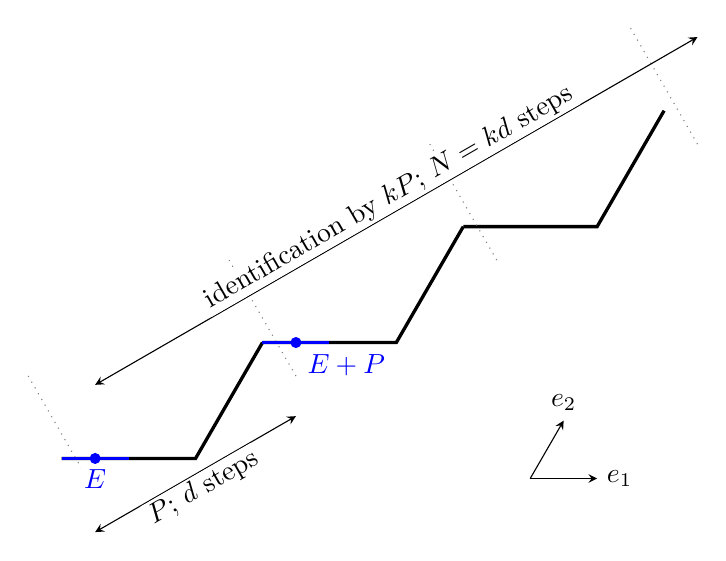
\begin{tikzpicture}[x=0.85cm,y=0.85cm,>=stealth]
  \foreach \j in {0,1,2} {
    \draw[very thick] ({3*\j},{1.73205*\j})
      -- ({3*\j+2},{1.73205*\j})
      -- ({3*\j+3},{1.73205*\j+1.73205});
    \draw[gray,dotted] ({3*\j+0.5},{1.73205*\j-0.5})
      -- ({3*\j-0.5},{1.73205*\j+1.23205});
  }
  \draw[gray,dotted] (9.5,4.69615)--(8.5,6.42820);
  \draw[very thick,blue] (0,0)--(1,0);
  \draw[very thick,blue] (3,1.73205)--(4,1.73205);
  \fill[blue] (0.5,0) circle (2pt) node[below=3pt,fill=white,inner sep=1pt] {$E$};
  \fill[blue] (3.5,1.73205) circle (2pt) node[below right=3pt,fill=white,inner sep=1pt] {$E+P$};
  \draw[<->] (0.5,-1.1)--(3.5,0.63205)
      node[midway,below,sloped,fill=white,inner sep=1pt] {$P$; $d$ steps};
  \draw[<->] (0.5,1.1)--(9.5,6.29615)
      node[midway,above,sloped,fill=white,inner sep=1pt] {identification by $kP$; $N=kd$ steps};
  \draw[->] (7,-0.3)--(8,-0.3) node[right] {$e_1$};
  \draw[->] (7,-0.3)--(7.5,0.56603) node[above] {$e_2$};
\end{tikzpicture}
\caption{A monotone staircase carrying the two identical translated marks.
The example has $P_1=P_2=2$ and $k=3$.  Translating the staircase in the
third edge direction produces the lozenge rows; the dotted segments
indicate that transverse direction.  The two background lists have
lengths $d$ and $N-d$ after adjoining one marked site to each.}
\label{u:staircase-figure}
\end{figure}


Use a row cut obtained by a periodic monotone staircase in \(e_1,e_2\) (period \(P\), passing through the marks), and translate it in the third lattice-edge direction to make rows. This tiles by lozenges with acute or obtuse angle at the corner between the increasing row and the transverse vector; drawing as square tiles, the same honeycomb path weights are given by \(R(t+v_i)\) at argument \(L\) or \(2L\), respectively (the two choices reflect the base angle, interchanging \(a,h\) and \(c,d\) in the tile notation). By lattice reflection if necessary take the majority steps to have argument \(2L\). The infinite-height projection and orientation argument for the two marks in the flip formula therefore apply verbatim to these physical column parameters (above, their negatives in the formula by crossing). For the use of the projection, lifted individual arches have summable mass and through-lines to height tending to infinity have vanishing mass at fixed \(N\). Indeed in the planar lifted slab or half-plane bounded by these stairs the contour from a fixed boundary source has a common rotated real coefficient bounded positively: turns to other boundary exits are given by cyclic outward-normal differences minus \(\pi\), with a single consecutive pair of lattice normals for the rounding, so only one sign of excess up to \(\pi/3\) is possible. Transversal pure cuts can truncate the sides. For decay cut further by a pure hexagon of radius comparable to height. Mass to the hexagon cuts is \(O_N(r^{-1/4})\): average over order \(r/N\) translations by whole periods putting the starts at distinct positions in the central part of a common smaller hexagon (contour subtraction before translating), and reverse at the pure sides to use their escape bound in a positive contour, with order \(r\) such exits. This is the flat-side argument of the geometric estimates. Thus through-line systems disappear by absolute single-path bounds and empty projections have the same limits.



For detail use lattice coordinates \((X,Y)\) along \(e_1,e_2\), with transverse step \(e_2-e_1\). Between transverse truncations (bounds on \(X+Y\)) and the two periodic stairs this domain has lower and upper bounds on \(Y\) as functions of \(X+Y\), both with slopes 0 or 1. Intersecting with pure hexagons or parallel pure half-planes (bounds on \(X,Y,X+Y\) at lattice levels) retains that same form: the bounds use maxima/minima, with feasible section on an interval since comparison with each affine bound uses monotonicity (of both stair coordinates). The CCW tangent directions thus occur in a lower block alternating directions 0,1, then possibly direction 2, upper block using 3,4, possibly direction 5 (units \(\pi/3\)). The cyclic tangent increase to exits from a given boundary midpoint therefore stays in either \([-\pi/3,2\pi]\) or \([0,2\pi+\pi/3]\), depending on the starting direction. Subtract \(\pi\) to get the path turn by boundary closure. This gives the asserted rotated positivity since \((3/8)(2\pi+\pi/3)<\pi\), and applies to subtraction of signed contours as before (terms on shared exits which stay inside agree). The planar flux rule still applies in these simply connected regions. To bound through mass from one stair in a wide truncation at fixed period, take a common lattice hexagon centered near that start of radius comparable to slab height but small enough not to reach the opposite stair. Start also at its period translates in the central part, and subtract the contour in the intersection to bound the individual through masses by the mass to the hexagon cuts. Upon reversal from each such new exit, cut again parallel to its pure side before the central targets; subtraction bounds their mass by that to the new line, at most a constant times the straight strip bridge sum at comparable scale. Letting the transverse truncations recede, the through masses are equal by periodicity. This gives the bound stated above. Arch sums themselves are bounded just by the positive contour, using exhaustion.



Both extra rapidities in each column now have the same value, denoted \(x_e\). The two common lists have sizes \(m=d-1,n=N-d-1\). Augment each for the plasma calculation by one site at \(x_e\), forming background lists of sizes \(M_A=d,M_B=N-d\), both even, now having identical proportions of the two possible values. In this section use \(\lambda_b=\pi/(2b)\); write \(\lambda\) for the proportion of minority steps, \(0<\lambda\le1/2\). By translation of rapidities we take the majority value to be \(r_0 L\) and the minority \((r_0-1)L\), where \(r_0=1/4+\lambda/2\).



The residue calculation starts from all common labels positive (whether neutral then or not), using its product as prefactor. Exactly as in the balanced two-leg case the potentials are now one copy of \(R_{g h}(i(w+i v_e))\) per augmented-list site \(e\) of color \(h\), value \(v_e\), and the common magnetic factor \(-\sinh(w+i x_e-iL)/\sinh(w+i x_e+iL)\); this follows by translation in each extra-slot factor of that calculation. Denote the remaining residue sum by \(P'\). The prefactor divided by \(f_N^2\) in the observable is
\begin{equation}
 \frac{C^{N/2}\prod_{e<f:\ g_e=g_f}D(v_e-v_f)}{2 f_N^2}
 \prod_{e\text{ common}} \frac{J(v_e-x_e)}{J(x_e-v_e)}
 \label{eq:legacy-P-23}
\end{equation}
by \(D(y)=J(y)J(-y)\), \(Q_{11}=C/2\). Elementary lowering counts satisfy \(K_g=M_g+u\) with common integer \(u\).



Periodize as before, using magnetic factor
\[
 U_T(w)=-\frac{S_T(w+i x_e-iL)}{S_T(w+i x_e+iL)}
 \left(e^{-3iL}\frac{S_T(w-T/2+iL)}{S_T(w-T/2+4iL)}\right)^2,
\]
and in the central theta sum include background charges \(q_e=-q_{g_e}\) at offsets \(a_e=-v_e\) (to avoid confusion, \(q_{g_e}\) itself denotes the color sign as for a particle). Thus \(X\) in the center Gaussian includes \(\sum_e q_e i a_e\). This ensures periodic differentials. Initially use rapidities near zero, so all contour openings and deformations work by continuation. The lift is still a finite sum analytic near nome zero, by split poles as before. At final rapidities differences \(L\) in the site lists one uses limits: before opening, the individual residue terms obtained by splitting have only denominators from the displayed shifted \(S_T\)'s and constants, independent of counts of sites except via multiplicities. Possible singularities at exact differences stay on the very same pair hyperplanes independently of nome on the small disk. Removability there for the lifted sum will also follow below by analytic continuation in rapidities of the final integral bounds (identity first for real periods). Thus maximum modulus at those values is permitted.



\subsection{The ordered magnetic gas}
\label{u:ordered-gas}

The staircase determines the background lists.  We next express their
residue sum as an ordered gas whose integer height records the winding.
Keeping the phases in this step is essential: the interval estimate below
uses the resulting transfer operator, not the absolute value of an
unidentified periodic partition function.

Here are details of extending the mode calculation. Put \(E(p)=\sum_e e^{-p a_e}{\bf e}_{g_e}\). In the mode matrix include extra background slots \(E_e\) with count-mode 1, pair entries from the potential factors (so \({\cal M}_{R,E}n_E=-K\widehat\rho E\)), inverse couplings to them initially zero. Their mutual block is zero except that formally at Laurent zero assign the pole terms
\(4q_eq_f/p^2+4q_e q_f(a_e-a_f)/p\), of zero finite part. Then:


\begin{itemize}

\item 

The bulk term in log is
\begin{equation}
 S(T)=\frac1{2T}\sum_p E(-p)^t K(p) E(p)\widehat\rho(p)^2
 -\frac12(T/3-2\log2)(M_A-M_B)^2.
 \label{eq:legacy-P-24}
\end{equation}
Determinants and measure conventions in \(\eqref{eq:legacy-P-star}\) are unchanged.



\item 

Chemical potentials per final particle (before adding the magnetic test) are
\begin{equation}
 2\pi i\,\sigma_i\sum_{e:g_e=g_i}
 \int_0^{s+i(v_e+\delta_i L)}\sum_{\nu\in\mathbb Z}\rho(z+\nu T)\,dz ,
 \qquad \sigma=(0,1,1,-1,0).
 \label{eq:legacy-P-25}
\end{equation}
Fugacity \(e^{-u r}\) if used still brings \(T r_j^2/(4h_*)-r_j(u_*+\bar L)\).
Indeed distribute \(2X^2\) into all pairs including background-background. The terms with \((a_i-a_j)^2\) in units of \(1/T\) again sum to \(-2 A_{\rm tot}^2\) with all charged offsets included; the missing constant logs from the background block give just the second term of \eqref{eq:legacy-P-24}. Thus the same verification by \(\gamma\) and its two charge conditions works with the extended block, including the center terms with \(l\); the Laurent saddle adds \(\widehat\rho E\) to the earlier residual saddle, giving the same common-integer Poisson sum and \eqref{eq:legacy-P-24}. In the chemical calculation the old simplifications apply in both color sectors individually: with \(H_V\) defined like \(H\) using multipliers \((0,-1,0,0,2c,0,0,-1)\), one has \((H_V+H\widehat\rho)(a;t)\) at \((0;0),(2;1),(2;-1),(3;-1)\) respectively \(0,0,\widehat\rho,0\). Insert the rapidity shift exponent to obtain \eqref{eq:legacy-P-25}. These formulas are for analytic continuation, so \(\sigma=0\) terms stay absent even beyond a primitive strip.



\end{itemize}


More explicitly at zero take the raw right count vector with left and inverse modes as before, appending background modes identically 1, and prescribe the same derivative condition \(q^t\gamma'_{\rm raw}=A_L+\sum_e q_e a_e+\pi l/2\). Then the second-order and first-order poles of the extended matrix still have the displayed charge/offset/winding form of the gas proof, so evaluation gives the actual center Gaussian and winding phases (including phase slopes from the potentials on left contours). The sum of charge products for pairs including real charges but not background-background alone is \(-\tfrac12(M_A-M_B)^2\) minus half the elementary count; regular diagonals treat the latter part as before. The additional saddle term \(\widehat\rho E\) neutralizes the appended charges at 0 and contributes exactly \(\sum_e q_e a_e\) to the derivative charge sum, while its count value \((M_A,M_B)\) leaves the free integer and Gaussian shift unchanged. The assigned background block has zero contracted finite part of its own. For \eqref{eq:legacy-P-25} the remaining linear symbol at a particle against each same-color site is \(-2\pi\sigma_i e^{(v_e+\delta_i L)p}\widehat\rho(p)/p\), yielding that primitive including the finite part at zero.



We describe the ordered-position form of the residual sum. Let \(\ell_{gi}\) count original left elementary members of species-color index \(i\) belonging to \(g\), write \(\ell_{\Sigma i}=\sum_g\ell_{gi}\). For particles in increasing order of real contours, write \(H(s)=j+\sum_{\Re s_d>\Re s} W_d\), \(j\) the Poisson integer; at a jump use its mid-value \(H_m\). Winding neutrality closes this integer path. Set the real row \(c^t\) by
\[
 {\bf1}^t(J(p)-K(p)\ell)=2\pi W^t/p-2h_* c^t+O(p).
\]
(In this expression \(J\) is the coupling block of the transform, transported on the final constituents, not the site function in \eqref{eq:legacy-P-23}.) Thus \(u_*+\bar L=c^t n-(\pi i/h_*)\sum W_d s_d\). At zero,
\begin{equation}
 Z=\alpha WW^t/p^2+M_*/p+O(1),\qquad
 M_*=-2\pi(\widetilde{\cal W}+W c^t-c W^t),
 \label{eq:legacy-P-26}
\end{equation}
where \(\widetilde{\cal W}\) is an integral skew matrix. Indeed change right variables by \(-\ell n\) in the block matrix before Schur. The non-right charges are now zero, its non-right block has simple coefficient \(-2\pi\widetilde{\cal W}\) from the shifted winding matrix (\({\cal W}_{nn}-\ell^t{\cal W}_{Rn}-{\cal W}_{nR}\ell\) before subsequent branch corrections). The remaining poles after Schur come just from the common channel as shown. Exact-offset averages for free left clusters give integral windings here (symmetric shifts for same offset clusters; otherwise all off singular offsets, even sum of multiplicities).



Apart from the explicit terms of \(\eqref{eq:legacy-P-star}\) and site/test couplings the constant phases, when \emph{combined} with the ordered factor from \(M_*/p\) and the term \(-2\pi i j c^t n\), reduce up to a single unit prefactor to
\begin{equation}
 \prod_d \eta_{i_d} \exp[-2\pi i c_{i_d} H_m(s_d)]
 \label{eq:legacy-P-27}
\end{equation}
for fixed unit constants per species, the same for every choice of even \(M_A,M_B\), including 0. Here and below indices in such products include the color. To check this, the \(1/p\) kernel at ordered separation is \(-i/2\) (positive separation), so neutrality gives the stated mid-value term and an unordered sign \((-1)^{\widetilde{\cal W}_{ab}}\) per pair. Before branch moves, original log constants have signs \((-1)^{{\cal W}_{ab}}\) on pairs of left particles, plus \((-1)^{\sum k_g P_g}\) from right-left pairs, where \(k_g=M_g+u-\sum_i\ell_{gi} n_i\) and \(P_g=({\cal W}_{R,L'} n_{L'})_g\); backgrounds contribute no sign (zero right winding, integral left windings and even counts near zero rapidities). Indeed for each shifted product of sinhs the positive-separation leading logs have just the offsets times \(i\), without extra signs before taking the indicated means and jump, since the products use symmetric shifts. Residue orientations can add single-cluster phases only. Original right and inverse same-side symmetrization gives exponents \(\sum_g\binom{k_g}2+\sum_{g,t}\binom{n_{gt}}2\), and the Weyl exponent adds \(\sum_g\lfloor(1-k_g-n_{I,g})/2\rfloor\), with \(n_{gt}\) inverse counts, \(n_{I,g}=\sum_t n_{gt}\). These are exactly the constant-mode signs in the trace calculation of \(\eqref{eq:legacy-P-star}\) (between different ordered oscillator radii the geometric log has zero constant phase). Dependence on \(u\) cancels since each simultaneous unit increment flips \(\sum_g(P_g+n_{I,g})=0\bmod2\). At \(u=0\) changing \(M_g\) by 2 also has no effect. Now on count space all second differences of this total sign exponent, mod 2, are precisely \(\widetilde{\cal W}\): in addition to the left-left and right-left terms, the binomials and floors (using \(\lfloor(1-h)/2\rfloor=\binom h2\bmod 2\) for integral \(h\)) contribute per group the polarization entries of shift type
\(\ell_g\otimes n_{I,g}+n_{I,g}\otimes\ell_g+n_{g+}\otimes n_{g-}+n_{g-}\otimes n_{g+}\) (symbols here denote linear count functions). These give the inverse-inverse and shifted right-inverse windings. This cancels the unordered signs from \eqref{eq:legacy-P-26}, leaving just single-particle phases. Each subsequent branch change of order \(\nu\) shifts \(\widetilde{\cal W}\) correspondingly and brings the matching constant sign \((-1)^\nu\) between the pair by the ratio of geometric factors as in the mode calculation. Fusion restricts to sums of constituents (self-residue has only a local extra phase), with the same compensation for exterior pair branch changes. This proves \eqref{eq:legacy-P-27}.



For the short part of pair energy we use the periodization of \(G_{ab}(s)\) for ordered positive separations (target to the right, source to the left), with the usual regular diagonal at contact and both periodic continuations counted, once per positively separated pair up to translations. This denotes the inverse Fourier kernel after removing exactly the two pole kernels in \eqref{eq:legacy-P-26}, with transpose at negative separations. Thus the off-contact exponent in the gas is minus one copy of \(G\) per such pair, including pairs with translated particles, and the regular contact self term with half weight. For \(\Re s>0\) we have
\begin{equation}
 G_{ab}(s)=\sum_{l\ge1}\sum_{k=0}^{r_*} C_{ab,l,k}s^k e^{-\omega_l s},
 \label{eq:legacy-P-28}
\end{equation}
where \(\omega_l>0\) increase at least linearly, \(C\) grow at most polynomially and \(r_*\) is fixed. Indeed the rational functions in the final symbols of the two-line calculation have only unit-circle poles in \(e^{Lp}\), of uniformly bounded order (the extra denominators after Schur come from \(H_*\), proportional in the channel symbol to \((1-e)(\coth(bp)-c\,{\rm csch}(bp))\), and use the earlier factorization of \(1-e\)). Shifting the inverse contour downwards in imaginary-period multiples picks these residues apart from the already separated zero pole terms. The horizontal ends can be bent down at small slope (symbols subtracted at zero are bounded or \(O(1/p)\) there); equivalently for the unsubtracted meromorphic symbol use a principal finite-part integral, whose zero pole contributes just the two displayed long kernels. Along deep level shifts chosen a fixed distance from poles the tail rotation yields exponentially vanishing remainder. This agrees at real periods with the ordinary periodized short kernel by Fourier inversion (at contact the one-sided short parts can have a jump; for the self entry there is no jump), and then by the continuation of \(\eqref{eq:legacy-P-star}\). More explicitly removing \(\alpha WW^t/p^2+M_*/p\) gives a symbol regular at zero, \(O(1/|p|)\) at either end, with inverse integrable at zero (log plus bounded terms). Its ordinary periodization includes the exact zero harmonic; the pole kernels separately are as in \eqref{eq:legacy-P-P3}.



\subsection{From periodic gas estimates to interval operators}
\label{u:interval-operator}

We next construct an operator whose products describe intervals of the
ordered gas.  This construction is needed because the magnetic core and
the two exterior intervals have different particle potentials.  A bound
on homogeneous closed periods would not by itself control their product.

Here is the required transfer estimate. Fix a large cell length \(S_0\); consider first a homogeneous gas with no magnetic functions or \eqref{eq:legacy-P-25}, but take \(r=-2a_0'\) constant, \(a_0'=+6Li\) or \(-6Li\), and allow all five species of color \(A\), only \(S,F\) of color \(B\). In addition to \(G\) and \eqref{eq:legacy-P-27} this has exponent
\begin{equation}
 -h_*^{-1}\int(\pi H+i a_0')^2\,ds
 + 2a_0' c^t n.
 \label{eq:legacy-P-29}
\end{equation}
The construction below will give a common state space for the two tilts; Lemma~\ref{lem:u-homogeneous-operator} then states the strict spectral bound.



\paragraph{Coercive gauge and nearest cells.}
We specify the operator since a pressure comparison on closed periods, without controlling intervals, would not suffice. A cell state \(x\) consists of the incoming integer height and indistinguishable points of each species/color in an open interval of length \(S_0\), with their factorial Lebesgue measure using the particle normalization of \(\eqref{eq:legacy-P-star}\). Include all species of both colors in the ambient space even if some are suppressed by zero point weights. Along an edge \(x\to y\) require outgoing height of \(x\) equals incoming of \(y\).

Use the real reference energy at zero tilt, no extra particle potentials: \(A(x,y)\) is half each of the two cell self energies (including \(\pi^2/h_*\int H^2\)), plus the real adjacent pair energy from \eqref{eq:legacy-P-28}. Cyclic sums omit just separations of at least two cells in \eqref{eq:legacy-P-28}. By \eqref{eq:legacy-P-P3}, for large fixed \(S_0\) they satisfy
\begin{equation}
 \sum A(x_i,x_{i+1})\ge 4\epsilon_S\sum_i |x_i|_0^2-C_S n_{\rm cells},
 \qquad |x|_0^2=N_x^2+H_{x,\rm in}^2 ,
 \label{eq:legacy-P-30}
\end{equation}
where \(N_x\) is total particle count, \(\epsilon_S>0\) at least inverse-polynomially small in \(S_0\). Indeed omitted terms cost exponentially small times \(\sum N_x^2\); interval counts in \eqref{eq:legacy-P-P3} control \(\sum N_x^2/(1+S_0)\), and incoming height is controlled by within-cell heights and counts. Here \eqref{eq:legacy-P-P3} at real large period is independent of the number of site sources; its proof holds for every large period. One may repeat a short cycle before applying it. Coincident points inside cells need not be used.



There is then a finite Borel real function \(\phi(x)\) on these states away from coincidences such that
\[
 A(x,y)\ge 2\epsilon_S(|x|_0^2+|y|_0^2)-C_S+\phi(y)-\phi(x).
\]
Indeed take the infimum of corrected path sums (subtract the count squares, add \(C_S\)) from an empty cell of height zero. There are finite paths both from the empty state to any prescribed
state and back, because jumps of both unit signs are available.  A fixed
return path and \eqref{eq:legacy-P-30} bound all corrected forward path costs from below;
a fixed forward path bounds their infimum from above.  The infimum is
therefore finite.  On each component with prescribed particle counts
and height, the energy is continuous away from coincidences.  Taking
intermediate positions in fixed countable dense subsets consequently
leaves the infimum unchanged and makes it a Borel function of the terminal state.

Gauge every forward transfer edge by \(\exp(\phi(y)-\phi(x))\). The gauge cancels on cycles. Complex nearest-cell weights use the same split into halves on self terms including the real reference height square, and all adjacent interactions as above; other point, height and oriented phase terms can be assigned wholly to the first cell on its outgoing edge. The gauge provides Gaussian margins in both endpoint states.

It still does so for small-slope complex deformations of the cells (holomorphic off null sets). Specifically compare curves parametrized over the same real intervals with derivative within a sufficiently small constant of 1 and with differences of successive position shifts Lipschitz-small, including across ends. The derivative of the short kernel away from 0 on that sector is bounded by \(C(1+1/|\Re s|)e^{-\gamma|\Re s|}\) by contour rotation as in \eqref{eq:legacy-P-P3}; self regular diagonal does not move. Thus local short comparison costs \(O_S(\text{slope error})(N_x^2+N_y^2)\). The height square has the same type of bound with also incoming heights; Jacobians can go into point weights.



\paragraph{Fock encoding of longer interactions.}
Encoding decaying pair interactions in a bosonic transfer space and recovering
periodic partitions from determinant-corrected traces has precedents in
one-dimensional spin systems~\cite[Sections~4--6]{HilgertRilke2008}.
Here the preceding gauge supplies the bounds needed for the unbounded
particle counts and integer heights.

For interactions of range at least two cells add a boson symmetric Fock space over countably many finite propagation blocks. They use semigroups \(D_d\) with each block generated by \(-\omega_l+\text{nilpotent}\), the nilpotent a bounded Jordan shift. Choose finitely many blocks per \(l\) and creation/detection arrays \(u_a,v_b\), with bilinear pairing in each block, so that
\[
 v_b D_d u_a=-G_{ba}(d)
\]
term by term in \eqref{eq:legacy-P-28}. The entries of these arrays need grow only polynomially in \(l\) before a rescaling; the unpropagated arrays need not be Hilbert-space vectors. Only the propagated sums below enter the Fock operators, and their square-summability will follow from the exponential decay. At edge \(x_i\to x_{i+1}\) the Fock state is passed from their common boundary to the next one; annihilate against \(V=\sum_{b\in x_{i+1}} v_b D_{d_b^L}\), where \(d_b^L\) is displacement within that cell from its left boundary. Propagate by \(D_{\ell'}\), \(\ell'\) the length (complex displacement) of \(x_{i+1}\); then create \(U=\sum_{a\in x_i}D_{\ell'+d_a^R}u_a\), \(d_a^R\) displacement from particle to right edge in \(x_i\). More precisely the Fock operator in forward order is
\[
 \exp a^\dagger(U)\ \Gamma(D_{\ell'})\ \exp a(V),
\]
with creation and annihilation in exponential-vector normalization, \([a(V),a^\dagger(U)]=VU\), and \(\Gamma\) symmetric tensor powers including vacuum.

By the rescaling \(u_a\mapsto e^{\omega_l S_0/3} u_a,\ v_b\mapsto e^{-\omega_l S_0/3}v_b\) modewise, \(\|U\|+\|V\|\le Ce^{-\epsilon S_0}(N_x+N_y)\). This Fock operator has trace norm at most \(C\exp(C\|U\|^2+C\|V\|^2)\). Indeed one can split \(\Gamma(D_{\ell'})=\Gamma(\tfrac12 I)\Gamma(4D_{\ell'})\Gamma(\tfrac12 I)\), with middle trace norm bounded by the convergent boson product of singular-value factors by strict summable contraction. Creation exponential times \(\Gamma(\tfrac12 I)\) is bounded as stated by its series (the \(k\)th power on degree \(m\) has norm at most \(\|U\|^k\sqrt{(m+k)!/m!}\)); likewise adjoint. Thus this cost is allowed within the Gaussian margins.

The resulting integral operators including the classical state on \(L^2\) are Hilbert-Schmidt. This remains true uniformly with bounded-above point log moduli per particle and bounded linear and constant perturbations of the volume height energies.



\begin{lemma}[Homogeneous interval operators]\label{lem:u-homogeneous-operator}
Choose $S_0$ sufficiently large and keep it fixed.  On the common
ambient cell space with Fock fibers constructed above, let
$\mathcal T_\pm$ be the homogeneous cell operators with all five species
of color $A$ and only $S,F$ of color $B$, the other species having zero
outgoing point weight.  There are no magnetic functions or potentials
\eqref{eq:legacy-P-25}; the constant tilt is $a_0'=\pm6Li$, $r=-2a_0'$,
and the weights consist of $G$, the phases \eqref{eq:legacy-P-27}, and
the exponent \eqref{eq:legacy-P-29}.  Then $\mathcal T_\pm$ are
Hilbert--Schmidt and their spectral radii satisfy
\[
 \operatorname{spr}(\mathcal T_\pm)<\exp(S_0/2).
\]
\end{lemma}
\begin{proof}
The construction proves the Hilbert--Schmidt assertion.  We prove the
spectral bound by identifying the cyclic traces and comparing two
representations of the same residue sum.

\paragraph{Cyclic traces and spectrum.}
Their ordinary traces of cyclic products (at least two edges) give exactly the ordered periodic gas times \(\det(I-D_T)^{-1}\), with \(T\) the whole period, this scalar tending to 1 at large period. In fact tracing the Fock product gives, besides this determinant, all contractions from previously propagated creations (also on earlier translates) into detections, hence sums precisely \eqref{eq:legacy-P-28} at positive separations of two or more cells, no others.

This identity follows simply by commuting exponentials, or Taylor-expanding on the occupation basis in finite blocks with the convergent geometric trace. In detail after multiplying into normal form \(e^{a^\dagger(P)}\Gamma(D_T)e^{a(B)}\) times its internal contractions, the normalized trace is \(\exp(B(I-D_T)^{-1}P)\). This follows by summing on each oscillator for diagonal \(D_T\), then for general strict contractions in finite dimension by conjugation on tensor powers and continuity; mode cutoffs converge by the bounds above. Internal and cyclic contractions then have the indicated time order.

The classical kernel trace formula with Fock fibers follows by Hilbert-Schmidt approximation, or composition and the Hilbert-Schmidt pairing (absolute kernel bounds Gaussian). For a homogeneous restriction suppressing species only by a point factor on outgoing sites the nonzero spectrum agrees with the restriction to allowed cell states, by block triangularity.



It suffices to bound homogeneous logarithmic trace per unit length on periods \(T=m_0S_0\), \(m_0\to\infty\). Indeed for a compact Hilbert-Schmidt operator the limsup root of absolute traces of powers is the spectral radius. For positive spectral radius one can split off by spectral projection the finite-dimensional outer eigenvalues with algebraic multiplicities; on the complementary invariant space smaller radius bounds even the power traces since two initial powers provide trace class. Leading eigenvalue powers cannot cancel at exponential scale along all integers (take simultaneous subsequences of phases tending to 1). We use here just the usual compact-operator spectral and spectral-radius facts (nonzero spectrum isolated poles of finite rank, \(\lim\|A^n\|^{1/n}\) equals spectral radius).



To bound those closed periods first fix real \(T\) large, and apply the two-line residue transform with \emph{no} magnetic potential, \(r=-2a_0'\), to backgrounds \(M_A=0,\ M_B\to\infty\) even with all variables zero. The original sum has no \(A\) particles because their original small residue contours have no site poles, and in particular only \(u=0\). Nevertheless opening and transforming both lines is still valid (coefficientwise proof as for \(\eqref{eq:legacy-P-star}\)). After removing \eqref{eq:legacy-P-24} the limit of the transformed gas keeps exactly the permitted species above, since nonzero \eqref{eq:legacy-P-25} on \(B\) have real part strictly negative proportional to \(M_B\) uniformly around this fixed real period. Dominated convergence follows from \eqref{eq:legacy-P-P3}. By \eqref{eq:legacy-P-26},\eqref{eq:legacy-P-27} and Coulomb integration the remaining exponent indeed has \eqref{eq:legacy-P-29}, since \(\int (H-j)=\sum W_d s_d\). Its determinant scalar per unit length in log is \(1/2+o(1)\).



\paragraph{The one-line comparison.}
The very same residue sum (without opening \(A\)) admits the one-right-line version of the current calculation on \(B\). Here are verification details. Use the heat period \(2bc_*\) with just one insertion in the normalized oscillator trace, \(K_{0,BB}=(2\pi/p)\coth(bp)\) and dressing factor \(1-e\) as before. A single Weyl reflection twists oscillator trace by oscillator sign, contributing the additional scalar \(\prod_{p>0}(1-e^{-2bp})/(1+e^{-2bp})\) and replacing Cartan covariance by \((p/2\pi)\tanh(bp)=K_{0,BB}^{-1}\). Indeed contractions run around with negative multiplier each time; the two inverse sides with the Cartan exponential then have evaluation multipliers \(-t e^{a_t p}\tanh(bp)\) including their own \(e^{-\phi}\), and the ordered inverse kernel uses this same \(\tanh(bp)\) in place of the reciprocal-channel multiplier, keeping the order subtraction in \(B(p)\). Equivalently these follow in \eqref{eq:legacy-P-P1} by moving the reflection to the end and replacing the oscillator occupation ratio in the one-line Wick contraction by \(-e^{-2bp}\) for \(p>0\). Gaussian integration again changes the reciprocal to that of \(K_{BB}\).

Zero momentum matching fixes \(q_B l=P_B+\sum t n_t\), allowing every choice of residual counts; the Laurent Schur saddle satisfies both charge conditions and no remaining mean Gaussian occurs (\(k_B=M_B-L_B\) fixed, \(Q\) vanishes quadratically at zero). Thus scalar \eqref{eq:legacy-P-24} is exactly the same; \eqref{eq:legacy-P-25} applies, and pair symbols through final fusion are precisely the given formulas with color entry \(c=0\), directly restricting original interactions to same color before Schur. Other zero factors have only polynomial growth in \(T\). All constant phase ambiguities here have unit modulus.



In slightly more detail, after moving the single reflection past the right inverse insertion the Cartan source has sign \(q_B\); relative to this sign the outer and inner inverse sources have signs \(-1,1\). Along the twisted oscillator trace the Cartan symmetric self contraction at harmonic \(\nu>0\) is \(\nu(1-h)/(1+h)\), \(h=e^{-2bc_*\nu}\), and ordered contractions use \(2\nu/(1+h)\), \(-2\nu h/(1+h)\); the momentum calculation at the insertion itself is unchanged. Thus even the inverse self terms have the same regular-diagonal convention (ordering singularity unchanged). Before the Schur step the Laurent pole matrices with winding are just restrictions of the earlier ones; the \(BB\) density block has leading \(4/p^2\), so its scalar equation at orders \(p^{-2},p^{-1}\) exactly enforces the count and derivative conditions against charge, leaving no order-zero quadratic correction. The twist product comes solely from the oscillator vacuum partition factor. No positivity of the twisted trace is being used.



For the analytic trace justification the preliminary inverse quadratic test from the two-line proof now has \(\Lambda=\tanh(bp)\), between the two tested values (the inequality is affine); all fixed-left convergence and subsequent termwise contour deformations therefore apply as there. The final same-color symmetric kernel is strictly positive with lower symbol bound \(\epsilon/(1+|p|)\), bounded real part at zero and high asymptotic \(2\pi I/|p|\).

We include the coefficient verification of positivity, since the one-line estimate is needed to control the operator on intervals. Take \(D_0(z)=(z^2-z+1)(z^4-z^2+1)\), \(t=e^{x/12}\), and \(H_{ij}=t^{-36+12(\delta_i-\delta_j)}D_0(t^{12})F_{ij}^{(0)}(t^{12})\), using \(x=Lp>0\). Clearing by positive scalars we want positivity of \((H+H^t)/(4\sinh x)\). Here \((H+H^t)/2\) is Laurent of degree at most 36 with coefficients at opposite powers negatives of one another (by substitution in the mode rules above). Let \(B_j\) denote its coefficient of \(t^j\), \(1\le j\le36\). Thus the matrix being tested is the sum of these with multipliers \(\sinh(\beta x)/\sinh x\), \(\beta=j/12\). As in the interpolation argument of \eqref{eq:legacy-P-P2}, with \(a=2\cosh x-2\) and nodes \(1,4,9\) the coefficients are
\[
 u_0=\beta,\quad u_1=\beta(\beta^2-1)/6,\quad u_2=\beta(\beta^2-1)(\beta^2-4)/120.
\]

For noninteger \(\beta\) the multiplier is between \(u_0+u_1a\) and \(u_0+u_1a+u_2a^2\) (divided differences of \(\sinh(\sqrt u x)/\sqrt u\) are positive by the power series); at integer arguments the latter is exact. Thus a Loewner lower polynomial has first two coefficients \(U_k=\sum_j u_k B_j\); its last is
\[
 U_2=\sum_j u_2 B_j-\tfrac12\sum_{12\nmid j}\left(u_2 B_j+|u_2|\operatorname{diag}(|B_j|_{\rm ent}{\bf1})\right),
\]
where absolute values inside diag are entrywise.



The finite coefficient check is as follows: multiplying by 1000, entries to nearest integers (error at most \(1/2\)) by substitution are, upper rows in succession separated by semicolons,
\[
\begin{array}{c|l}
0&1000,708,-958,625,1500;\quad2000,167,-667,1333;\\
 &2000,-1667,-1750;\quad2000,1333;\quad3000\\
 1&2000,827,-1385,684,1818;\quad4000,1327,-1920,1673;\\
 &4000,-2809,-2031;\quad4000,1673;\quad4000\\
 2&565,54,-210,26,146;\quad511,105,-146,166;\\
 &359,-175,-130;\quad468,166;\quad388
\end{array}
\]
For example one rule to obtain the entries is to clear each \(F^{(0)}_{il}\) by \(D_0\); place half each resulting coefficient at degree \(h\) in the bins \(j=12(h+\delta_i-\delta_l)-36>0\) of entry \(il\), adding the same with indices exchanged, before using the three displayed polynomials in \(j/12\).

Subtracting \(3I\) from each displayed integer matrix gives positive
successive leading determinants by rational elimination.  Each rounding
error has magnitude at most $1/2$, so its $5\times5$ matrix has operator
norm at most $5/2$.  Thus the exact matrices $1000U_k$ are positive
definite as well.  This proves positivity of all three $U_k$ without
using the rounded entries as exact coefficients. This yields the asserted bound near zero and strict positivity throughout; the limit after multiplying by \(p/(2\pi)\) at infinity is identity directly from the branch constants. The same smoothing/removal of regular diagonals used for \eqref{eq:legacy-P-P3} now gives absolute convergence and uniform domination for the limit in \(M_B\) at fixed period.



Again only \(S,F\) survive. Their symmetric entries, omitting \(2\pi/p\), on the diagonal are
\((\sinh3x+\sinh x\mp\sinh2x)/\cosh3x\) respectively, and off-diagonal
\((\sinh(5x/2)+\sinh(x/2))\cosh(x/12)/\cosh3x\).
Spatial real kernels are nonnegative off contact (each divided by \(p\) is a nonnegative mixture of \(\cosh(h p)/\cosh(bp)\) for \(0\le h<b\), with positive inverse transforms).

Regular diagonal of each whole-line kernel is at least \(2\log L\), since the diagonal multipliers \(F\) are both at least \(1-e^{-x}\) for positive \(x\) by substitution, and the regular value is \(2\int_0^\infty(F(e^x)-1+e^{-x/L})\,dx/x\) in notation where \(F\)'s argument is \(e^x\). Periodization only improves it. Hence the total real pressure from particles is at most \(1/(\pi L)\).

The one-line determinant per length gives \(1/4-1/6+o(1)=1/12+o(1)\) (expand the logarithms of the product above and one copy of \((1-e)^{-1}\)). Comparing both limiting expressions, the desired homogeneous log trace per unit length is at most
\[
 1/(\pi L)+1/12-1/2+o(1)<1/2.
\]
This proves the strict spectral bound for either sign of the tilt.
Indeed $L=\pi/8$ and $\pi>3$ give
\[
 \frac1{\pi L}+\frac1{12}-\frac12
 =\frac8{\pi^2}-\frac5{12}
 <\frac{17}{36}<\frac12.
\]
Thus the comparison has a fixed positive margin for both choices of
the tilt.
\end{proof}

For later use, the spectral-radius formula gives a fixed block length
$q$ and $\varepsilon>0$ for which both homogeneous operators satisfy
$\|\mathcal T_\pm^q\|\le\exp[(1/2-\varepsilon)qS_0]$.
Continuity of a finite ordered product in operator norm then preserves
the bound $\exp(qS_0/2)$ for sufficiently close $q$-blocks in the same
state space and gauge.  Section~\ref{u:core-product} will prove this
closeness for the actual tail kernels; the core requires its separate
product estimate.



\subsection{Localization of the magnetic source}
\label{u:magnetic-localization}

The homogeneous interval operator is now controlled.  We turn to the
actual magnetic source, prove the uniform one-particle estimates needed
to compare its tails with that operator, and retain the suppression
inside the shorter core.  Write \(a(s)=\log U_T(s)\) on the right contours, using the branch whose bulk core log comes from the odd primitive in the centered argument \(s+i x_e\); its total winding around the period is zero as in the balanced calculation of Section~\ref{c6:subheading-16}. All logarithms in exponents are continued along the stated graphs. As there, the right mean of \(a\) gives \(r=-2\bar a\) and scalar \((M_A+M_B)\bar a\); on the left retain direct \(U_T\) factors and subtract the mean, on the right transform insert \(a-\bar a\). Completing Cartan nonzero modes exactly as in the balanced case gives the following additional external scalar (in addition to \eqref{eq:legacy-P-24}, with the squared linear-primitive effect assigned below):
\begin{equation}
 S_a(T)=\frac1T\sum_p \widehat\rho(p){\bf1}^t E(-p)\widehat a(p)
 +\frac1T\sum_{p\ne0}\big(Q_+(p)-1/h_*\big)\widehat a(-p)\widehat a(p).
 \label{eq:legacy-P-31}
\end{equation}
The local height-square exponent is now again
\begin{equation}
 -h_*^{-1}\int (\pi H+i a(s))^2\,ds .
 \label{eq:legacy-P-32}
\end{equation}
Indeed the added particle-source nonzero-mode multiplier is 
\[
 -J(-p)^t{\bf1}Q_+(p);
\]
 its simple pole \(+2\pi W/(p h_*)\) acting on \(a-\bar a\) provides the corresponding mean-zero primitive of \(-i(a-\bar a)\). Summing jumps evaluates it by parts against \(H\); remaining terms here are exactly the long quadratic from \eqref{eq:legacy-P-26}, mean/fugacity tilt and the part of the test variance not kept in \eqref{eq:legacy-P-31}. The extra exponent at each particle, besides \eqref{eq:legacy-P-27}, consists of:
\begin{equation}
 (2c_i-\ell_{\Sigma i}) a(s)+\sum_{\text{orig. left members there}} \log U_T(s+i(\delta_i+b_{i'})L)+ b_i'(s).
 \label{eq:legacy-P-33}
\end{equation}
Here offsets \(b_{i'}\) denote the indicated individual physical integer additions. The short source \(b_i'\) is the Fourier action on \(a'\) of
\[
 [-J(-p)^t\allowbreak{\bf1}Q_+(p)-2\pi W/(p h_*)-(2c-\ell_\Sigma)]_i/(-ip),
\]
regular at 0. Indeed the definition just before \eqref{eq:legacy-P-26} gives the indicated constant coefficient \(2c-\ell_\Sigma\) using \(Q_+=1/h_*+O(p^2)\). Its mean times the counts comes from \(-\bar a \ell_\Sigma^t n+2\bar a c^t n\) in the left and fugacity terms; likewise the tilt with the mean of \(a\) in \eqref{eq:legacy-P-32} uses \(\int(H-j)=\sum W_d s_d\). Direct left log terms just mean products with their integer multiplicities.



Keep the cell length $S_0$, block length $q$, and spectral margin chosen above fixed. Choose the bend size $\theta_0$ sufficiently small, then the transition length $A$ and buffer $g\gg S_0$ sufficiently large to meet the slope bounds below. The fixed boundary layers used in the product estimate may depend on these choices, but none of these constants depends on $d,N$, or $\lambda$.

Take nominal period \(R=2a_0^{-1}\log N+g+O(S_0)\), a multiple of \(2S_0\), with \(a_0=\pi/b\) as in the gas calculation. Allow \(|T-R|<\pi+1\). Use a common curve for the positions parameterized by
\(s=t+i y(t)+(T-R)\chi(t)\), \( -R/2\le t\le R/2\), with the analytic period adjustment \(\chi\) as in \eqref{eq:legacy-P-P3}, derivative \(O(1/g)\), supported near the ends within \(g/3\), \(\chi(\pm R/2)=\pm1/2\). Use the periodic, real, Lipschitz-small displacement \(y(t)\) zero for \(|t|\le A\), decreasing in \(|t|\) to a fixed tiny negative constant \(-\theta_0 L\) by \(|t|=2A\), then flat (\(A\) large absolute, \(\theta_0>0\) sufficiently small). Slopes meet all earlier smallness requirements.



Here are uniform bounds on site sources on this graph:


\begin{enumerate}

\item 

\(a(s)\) tends exponentially to \(a_\pm=\pm6Li\) away from 0 and the period edges, on \(\pm t>0\), and is bounded. Logs in \eqref{eq:legacy-P-33} from direct multipliers likewise tend to these phases modulo \(2\pi i\), with multipliers bounded. The short \(b_i'\) tends exponentially to 0 there with \(\exp(\Re b_i')\) bounded throughout.



\item 

For \(D,I'_+\) the real exponent in \eqref{eq:legacy-P-25} is bounded above by \(-c_0 M_g e^{-a_0|t|}+O(1)\) with \(c_0>0\); the same estimate holds for \(I'_-\) when \(|t|\ge 2A\), and an upper bound \(O(1)\) everywhere. Moreover for color \(A\) the \eqref{eq:legacy-P-25} multipliers tend uniformly to 1 far outside \(|t|\le a_0^{-1}\log d\) and away from the period edges.



\end{enumerate}


For 1, the product formula and derivative periodizations about the two centers are as in the balanced case. Direct left physical offsets have no poles along the graph (the edge compensator unshifted in rapidity). For the short term apply the regular multiplier on the two separate whole-line coth derivative differences before periodization; their transforms off zero decay at the nearest respective shifted singularity, by integrating across one coth period. Products for the core have exponential decay in frequency (also on slightly bent shifted contours for spatial transport) uniformly in the shifted rapidities: the rates are controlled by \(1\mp(x_e/L+\delta_i)\); in a limiting case at \(S\) with positive frequency use the additional exponential decay of \(A_0(e^{Lp})\) there. For \(I'_-\) with negative frequency, isolate from \(b_i'\) for this core part only the multiplier \(-(e^{\delta_i Lp}-1)/(-ip)\). This gives minus the core log difference on shifting the argument by \(i\delta_i L\); its exponential modulus is bounded above (a possible approach is to the pole, not the zero, of the shifted ratio) and it is localized exponentially including its images. After this subtraction the extra exponent has uniform frequency decay since \(A_3=-1\). These statements use \(a'\) itself split as periodized whole-line differences around the centers (the opposite masses cancel globally). Contour rotation away from the centers as in \eqref{eq:legacy-P-P3} gives all asserted periodized bounds and continuation; for the isolated log difference use direct transport, with the limiting approach to a singularity only near \(t=0\) where the graph is undisplaced. Widths for the unshifted ratios in such estimates are bounded away from singularities since \(-3/4\le x_e/L\le1/2\).



For 2, images and period adjustments cost \(O(1)\) by exponential decay and the choice of period. On the basic line the imaginary part for a single primitive at argument \(t+iLY\) is
\[
 B(u,Y)=\frac1{2\pi}\operatorname{atanh}
 \frac{4\sqrt3\cosh u\sin(\pi Y/3)}{3+4\sinh^2u+4\sin^2(\pi Y/3)},\qquad u=a_0 t ,
\]
by integration of the explicit density. Before bending, take the mixture of \(Y=r_0+\delta_i,Y-1\) with proportions \(1-\lambda,\lambda\). For \(I'_+\) its sign is uniformly positive with size at least constant times \(e^{-|u|}\): \(Y\ge2/3\) and the positive function increases on \(0<Y<1\). For \(D\), \(Y=1/3+\lambda/2\); the same follows by monotonicity and continuity (including as \(|u|\to\infty\) after scaling) if \(\lambda\ge1/3\). Here are convenient comparisons for the remaining cases: on \(0<Y<1\), \(2\pi B\) divided by \(4\sqrt3\cosh u\sin(\pi Y/3)/(3+4\sinh^2 u)\) lies between 1 and \(\operatorname{atanh}(\sqrt z)/\sqrt z\), \(z=4\sin^2(\pi Y/3)/(3+4\sinh^2u)\). Indeed compare the argument of atanh to \(\sqrt{3z+z^2}/(1+z)\) below (the atanh at this lower value is at least \(\sqrt{3z+z^2}\) by differentiation, and atanh divided by argument increases) and \(2\sqrt z/(1+z)\) above. Thus for \(D,\lambda\le1/3\) the required margin follows from
\[
 (1-\lambda)\sin(\pi Y/3)-1.33\lambda\sin(\pi(1-Y)/3)>0
\]
The split at $\lambda=1/4$ makes this a quantitative comparison.
For $0\le\lambda\le1/4$, use
$\sin(\pi/9)>1/3$ and $\sin(2\pi/9)<2/3$; the displayed difference is
at least $17/600$.  For $1/4\le\lambda\le1/3$, use
$\sin(11\pi/72)>9/20$ and $\sin(13\pi/72)<11/20$; it is at least
$337/6000$.  The factor $1.33=133/100$ is valid throughout these
comparisons: the relevant $z$ is at most $5/9$, and
\[
 \frac{\operatorname{atanh}\sqrt z}{\sqrt z}
 \le 1+\frac z3+\frac{z^2}5+\frac{z^3}{7(1-z)}<\frac{133}{100}.
\]
For \(I'_-\), \(Y=\lambda/2\le1/4\), so $z<1/10$ and the same series
bounds the upper-comparison factor by $11/10$.  Moreover
\[
 \frac{11}{10}(1-\lambda)\sin(\pi\lambda/6)
 \le \frac{11\pi}{60}\lambda
 <\lambda\sin(\pi/4)
 \le \lambda\sin(\pi(1-Y)/3).
\]
This yields the negative sign with a fixed margin times
\(\lambda e^{-|u|}\). At large \(|t|\) bending down only improves that comparison, giving an absolute margin at full bend: \(B/e^{-|u|}\) there is uniformly increasing with slope bounded below on the needed interval by the displayed formula. Other comparisons are unaffected for small \(\theta_0\). This proves the suppression bounds. The real-axis primitive limits to \(\pm1/2\), unchanged on bounded parallel displacements with exponentially small error; in the last assertion of 2 the masses \(M_g\) are even. These arguments use analytic continuation on horizontal graphs first (\(|r_0+\delta_i|,|r_0-1+\delta_i|<1\) for nonzero \(\sigma_i\)) and the bend only far from core poles.



These estimates justify the mode transform at the indicated rapidities. More explicitly start at real large \(T\), near zero rapidities, where the analytic test can be taken through the original trace and the final fusions without pole problems, exactly as in the balanced case. Continue rapidities linearly to the targets on the final contours with horizontal projections (no remaining branch crossings in the continued \eqref{eq:legacy-P-25} or magnetic terms); absolute convergence throughout and in neighborhoods for fixed parameters follows by \eqref{eq:legacy-P-P3} or \eqref{eq:legacy-P-30}, since only bounded one-body and at most linear height perturbations are added. For the lift, split poles initially near the fictitious background only for \emph{actual} remaining residue sites, as in the balanced magnetic calculation (including common sites possibly colliding with those extra values); this gives meromorphic continuation with a finite product-sum representation. The straight continuation just given implies regularity there on the rapidity family used, even at collision divisors where the individual split terms need limits. Now deform the final position graphs to include the small \(y\) at real periods by simultaneous transport (contact repulsions have fixed continuation on the shared small-slope curve; long ordered factors can equivalently be reassembled in their analytic pair branches; no one-body singularities are crossed). This can also be done termwise before resumming the Poisson index by using each original Fourier coefficient for periodicity. Equivalently the Coulomb and mid-jump rules are local on the cyclic integer path, so after summation boundary terms always reindex periodically. Coincident loci have no poles, only possible zeros of nonnegative integral order with analytic transport, by the high-frequency coefficients. Uniform absolute convergence on the deformation follows as in \eqref{eq:legacy-P-P3}. Holomorphic continuation in the period disk then holds on the indicated parametrization, locally also for rapidities near the targets. Any singularities from split residues in taking those target rapidities at finite nome are on fixed rapidity divisors by the product rules at large \(\Re T\), hence the real-period regularity removes them identically near nome zero (analyticity in nome of the desingularized finite expression). Its value at zero is the original trigonometric sum, likewise by continuation. We thus bound on the nome circle using this common graph. Parameters can be kept on a full fugacity period when coefficient verification is needed.



\subsection{A bounded product through the core and tails}
\label{u:core-product}

Choose \(u_0\) a nonnegative cell-boundary coordinate within bounded distance of \(a_0^{-1}\log d\). On the core \([-u_0,u_0]\), where \(\chi=0\), remove the scalar \(h_*^{-1}\int a^2\) from \eqref{eq:legacy-P-32}, of real part \(-2(2u_0)+O(1)\), since \((6L)^2/h_*=2\). Redistribute the principal real linear tilt on that interval using
\[
 \int_{-u_0}^{u_0}\operatorname{sgn}(t) H(s(t))\,dt
 =-\sum_{d':\, |t_{d'}|<u_0} W_{d'}(u_0-|t_{d'}|).
\]
It appears with positive coefficient \(12\pi L/h_*\); terms from purely imaginary tangents here have unit modulus for this leading tilt. The unfavorable sites all have \(W<0\) and thus the strong chemical suppression, which absorbs their loss at bounded additive cost per particle while retaining an overall suppression \(-c_1(u_0-|t|)\) per particle there (\(M_g\ge d\), and no species has \(W=0\)). Here we actually replace that real part of the tilt in the local edge weights on the core by the point terms from the displayed identity; their cyclic product is unchanged. All other added terms have bounded-above point log moduli by 1 and 2, and at most bounded linear height costs on cells, whose real coefficients beyond the reference Gaussian tend to zero away from the center after this redistribution. There is no winding boundary cost in this telescoping.



Every edge kernel is uniformly bounded after the scalar removal.
We need the stronger assertion that the product through the whole core
has bounded norm, independently of its length.  We prove it directly.
For a core cell let its depth be its minimum distance from the two core
cuts, truncated below at zero. Reserve a fixed small fraction of the
remaining negative point potential $-c_1(u_0-|t|)$: on cell $i$ this gives
an outgoing factor $\exp[-p_i(x)]$, where
$p_i(x)=\delta\,\mathrm{depth}_i N_x$ for a fixed $\delta>0$.
Set $p_i=0$ on the exterior states at the two core interfaces. If
$K_i(x,y)$ is the outgoing edge kernel, replace it by
\[
 K_i^{\rm sym}(x,y)
 =\exp\!\left[\frac{p_i(x)-p_{i+1}(y)}2\right]K_i(x,y).
\]
The reserved factor on this edge becomes
$\exp[-p_i(x)/2-p_{i+1}(y)/2]$. In a product through the core the
multipliers telescope pointwise, including the interfaces where the
exterior factors are one. Thus the complete product kernel is unchanged;
no boundedness of an inverse diagonal gauge is required. Adjacent cell
depths differ by at most the fixed cell length. The unused point
suppression and the Gaussian margins in \eqref{eq:legacy-P-30} therefore
remain available on both incident edges. In particular, every block
with a nonempty state at either endpoint has operator norm at most
\[
 C\exp(-c\,\mathrm{depth}),
\]
where $\mathrm{depth}$ is the smaller of the two incident cell depths.
Here an empty state means no particles in the cell; its integer height
and Fock state are still retained.

Away from a fixed number of cells at the central transition and the two
cuts, the empty-to-empty block has norm at most one.  Indeed the integer
height is constant across such an edge and the real reference exponent
is $-\pi^2 S_0 H^2/h_*$.  The residual linear coefficient of $H$ tends
exponentially to zero away from the transition and the cuts.  Since
$H$ is an integer, its absolute contribution is then bounded by the
negative quadratic term whenever $H\ne0$; for $H=0$ both contributions
vanish.  The common tangent is flat there, the remaining scalar phases
have modulus one, the state gauge cancels, and the free Fock propagation
is contractive.  The complete edge consequently has norm at most
$1+C\exp(-c\,\mathrm{depth})$ on each of the two core halves outside
those fixed exceptional layers.  The sum of these errors is bounded:
for each depth there are only a bounded number of cells.  Taking the
product proves a uniform bound on the core operator.  The exceptional
layers contribute only fixed factors.  We use the redistributed gauge
only on core cells; the tail operators retain their original gauges.

On each of the two tails outside the core, far from its end cuts and the period edges, \eqref{eq:legacy-P-32},\allowbreak\eqref{eq:legacy-P-33} and \eqref{eq:legacy-P-25} converge in the same edge-kernel sense, uniformly, to the homogeneous kernels with \eqref{eq:legacy-P-29} and phases \eqref{eq:legacy-P-27}, since all undesired \(B\)-species are suppressed, and points on \(A\) see the chemical limit 1. The direct left factors with the displayed linear term in \eqref{eq:legacy-P-33} give exactly \(\exp(2a_\pm c_i)\). Pair kernels are unchanged on the interior flat cells (their common displacement cancels). Convergence in Hilbert-Schmidt norm as distances increase follows by bounded-state truncation and the Gaussian majorants. Use the fixed block length $q$ chosen after Lemma~\ref{lem:u-homogeneous-operator}, for which each homogeneous $q$-fold product has norm at most
$\exp[(1/2-\varepsilon)qS_0]$. Increase the fixed boundary layers
until the $q$-fold products of the actual tail edges differ in norm
from their homogeneous products by less than the available fixed
margin.  Their norms are then at most $\exp(qS_0/2)$.  The boundary
layers and the fewer than $q$ remaining edges have bounded length and
bounded norms.  Consequently the two tails together contribute at
most \((R-2u_0)/2+O(1)\) to the logarithm of the product norm. Short intervals and all remaining boundary layers need only the uniform edge bounds. In the cyclic trace estimate keep two edges in Hilbert-Schmidt norm to use the remaining product bounds. Including the core scalar but excluding \eqref{eq:legacy-P-24},\allowbreak\eqref{eq:legacy-P-31} and determinant, we obtain overall log modulus at most
\begin{equation}
 -2R+\tfrac52(R-2u_0)+O(1).
 \label{eq:legacy-P-34}
\end{equation}



\subsection{Matching the scalar and the Pfaffian normalization}
\label{u:marked-denominator}

The interval bound controls the particle integral.  To recover the
polygon observable we must still match its scalar factors with the
normalizing polynomial $f_N^2$.  This step is necessary even when the
staircase uses only two rapidity values, because those values may have
arbitrarily unequal multiplicities.

We first match the external scalars. Uniformly on the circle, \eqref{eq:legacy-P-24} equals
\[
 \tfrac12\sum_{e,f} I_{g_e g_f}(v_e-v_f)+C_2 e^{-2T}+O(1)
\]
for a constant \(C_2\) depending on the site data. Here
\[
 I_{gh}(v)=2 q_g q_h\log2+\int_{\mathbb R}\!
 [K_{gh}(p)\widehat\rho(p)^2\cosh(vp)-4q_g q_h/p^2]\,\frac{dp}{2\pi}.
\]
Indeed the subtracted pole all-mode sum is \(q_g q_h T/3\). The ordinary regular-symbol periodization picks corrections from poles at \(\pm2i\) and an error \(O(N^2 e^{-a_0 \Re T})\), by contour shifting with exponentially bounded tails; there is at most a simple pole at \(\pm i a_0\) also in the color difference channel by substitution. We have
\begin{equation}
 e^{I_{gh}(v)}= B(v)^2\tan^2(\lambda_b v)
 \begin{cases}1/D(v),&g=h,\\ 1,&g\ne h,\end{cases}
 \qquad B(v)=\sin(v+b)\sin(v-b)/\sin v .
 \label{eq:legacy-P-35}
\end{equation}
To verify, first take the difference from \(v=0\). Indeed with \(t=e^{-Lp}\) the multiplier \((p/2\pi)K_{gh}\widehat\rho^2\) on \(p>0\) is \(t^2/[(1-t+t^2)(1-t^8)]\) times \(1+t^6\) or \(-2t^3\) on same or opposite color respectively. Thus it expands as \(\sum_{k\ge1} c_k e^{-kLp}\) with
\[
 c_k=-2{\bf1}_{k=\pm3(8)}+2{\bf1}_{k=0(8)}+2{\bf1}_{k=3(6)}-2{\bf1}_{k=0(6)}
 +{\bf1}_{g=h}{\bf1}_{k=\pm2,\pm3(8)} .
\]
Integrating gives the sum of \(-c_k\log(1-v^2/(kL)^2)\), exactly the log ratio by the sine product. To fix the constant use \(v=i V\), \(V\to+\infty\) along the analytic convolution strip: by the pole transform and the integrable regular remainder \(I=2q_gq_h(\log2-V)+o(1)\), matching \eqref{eq:legacy-P-35}.



Formula \eqref{eq:legacy-P-31} equals
\[
 \sum_e\log\frac{J(x_e-v_e)}{J(v_e-x_e)}
 + C_1 e^{-T}+O(1).
\]
The regular test variance part costs \(O(1)\) as in the balanced magnetic calculation of Section~\ref{c6:subheading-16} (\(a'\) localized and analytic near the right graphs). The cross part integrates \(a\) against the shifted periodized densities (here one can use the centered straight period segment, slightly sloping for complex periods). The log of the normalized squared edge ratio gives first terms \(e^{-T}(d_1 e^{2s}+d_2 e^{-2s})\) across the core with constants \(d_1,d_2\), with bounded error \(O(e^{-2\Re T+4|\Re s|})\) (product expansion; the same error bound covers the distant images in the core log); their integrals against each nonperiodized density \(\rho(s+i v_e)\) give the coefficient, all tails/images and errors after summation costing \(O(1+N e^{-a_0\Re T/2})\) since \(2<a_0<4\). The remaining principal integral per background is the whole-line core-log convolution shifted by \(i(x_e-v_e)\). The derivative of that convolution has transform
\[
 2\pi i\widehat\rho(p)\frac{z-z^7}{1-z^8}
 =2\pi i\frac{z^2+z^3-z^5-z^6}{1-z^8},\qquad z=e^{-Lp},
\]
obtained from the localized coth difference. Thus the convolution itself is \(\log[J(-is)/J(is)]\) at \(s=i(x_e-v_e)\): the derivative there has the same transform by shifting across a coth period, and both functions are odd. Contours can be displaced within this convolution strip by keeping the two sets of poles separated (the absolute shift in the difference is at most \(L\), individual right displacements strictly inside their strips).



Use maximum modulus after removing \(C_2 e^{-2T}+C_1e^{-T}\) by an exponential analytic multiplier. The determinant in the two-color transform adds
\((3/8)\log N+O(1)\). To retain the bounded remainder, put
$\mathfrak d(p)=-\log(1-e(p))$ and write its logarithm exactly as
\[
 2\sum_{n\ge1}\mathfrak d(2\pi n/T)
 =\sum_{n\in\mathbb Z}\mathfrak d(2\pi n/T)-\mathfrak d(0).
\]
The symbol $\mathfrak d$ is even, regular at zero, and exponentially
decaying. Its inverse transform at nonzero period translates is
exponentially small, by a fixed contour displacement and bending of
the tails. Periodization therefore gives
$\pi T/(16L)-\mathfrak d(0)+O(e^{-c\Re T})$, as in the two-line
calculation. The two square-root factors have constant product.
Since $\Re T=(3/4)\log N+O(1)$, the real part gives the stated bound
uniformly on the nome circle. Formula \eqref{eq:legacy-P-35}, with \(e^{I_s(0)/2}=\lambda_b/\sqrt C\), cancels the all-positive prefactors in \eqref{eq:legacy-P-23} along with the site sum from \eqref{eq:legacy-P-31}, leaving exactly \(2 f_N^{(0)2}\) in the numerator relative to \(2 f_N^2\), where superscript \((0)\) indicates using \(h_0(v)=-\lambda_b\tan(\lambda_b v)/2\) instead of \(h\). This follows also by the Schur Pfaffian product at shifted variables as in the homogeneous calculation.



We need
\begin{equation}
 \log\big(f_N^2/f_N^{(0)2}\big)\ge (5/24)\log N-O(1)
 \label{eq:legacy-P-36}
\end{equation}
for these rapidities uniformly. Here is a shifted comparison. Temporarily center the variables in \([-L/2,L/2]\) and make them distinct (or perturb into a slightly larger interval). The kernels by their partial fractions are integrations of \(-\sinh(vp)\) against the two positive-ray pole densities \(\nu_0,\nu\) from the determinant comparison, ratio \(R(p)=\nu/\nu_0\ge1\). Expanding a Pfaffian of size \(N=2s\) by antisymmetry therefore gives the integral of the exponential alternant on exponents \(\pm p_1,\ldots,\pm p_s\) against the corresponding product measure, up to common constants. One may cut off at 0 before taking limits by entries. This alternant has fixed sign for distinct ordered variables when exponents are laid out in pairs (pair swaps do not change sign), since exponential polynomials of \(N\) such distinct exponents have at most \(N-1\) distinct real zeros by Rolle induction. Jensen thus bounds the log Pfaffian ratio below by its linear statistic with \(g=\log R\) in the \(h_0\) ensemble, equivalently the log derivative of \(\operatorname{Pf}(h_0+t h_g)\) at zero, where \(h_g\) uses pole density \(g\nu_0\). Limits at coincidence preserve this comparison by confluent determinants.



The doubled linear statistic has the form $A\log N+O(1)$, with a constant $A$ independent of the rapidities and of the even size $N$. We verify this uniform assertion before using coincidence to identify a lower bound for $A$. Write
\[
 H_t=\big[h_0(v_i-v_j)+t h_g(v_i-v_j)\big]_{i,j=1}^N,
 \qquad C(v)=\prod_j[-i\cot(\lambda_b(v-v_j))].
\]
If $\Gamma$ positively encircles the distinct sites and initially no
other poles, Schur's product and its minors give the exact identity
\[
 2\left.\frac{d}{dt}\log\frac{\Pf H_t}{\Pf H_0}\right|_{t=0}
 =-\frac4{(2\pi i)^2}\int_\Gamma\!\int_\Gamma
 C(v)C(w)h_0(v-w)h_g(v-w)\,dv\,dw.
\]
For the coefficient, put $r_i=\operatorname{Res}_{v=v_i}C(v)$.
Cancelling factors not incident to the two removed sites in each Schur
minor gives the undoubled derivative as
$-4\sum_{i<j}r_i r_j h_0(v_i-v_j)h_g(v_i-v_j)$.
The normalized double integral equals
$2\sum_{i<j}r_i r_j h_0(v_i-v_j)h_g(v_i-v_j)$; its diagonal-site
residues vanish because both kernels are odd. Doubling the derivative
therefore gives the displayed coefficient $-4$, independently of the
sites and of every even $N$. The odd function \(h_g\) is bounded analytic on strict substrips \(|\Re v|<5L\), by exponential decay of \(g\nu_0\); at frequency zero the density may have a constant times \(1/p\), whose odd sine integral with cutoff remains bounded. Expand first the \(v\) contour to a rectangle of vertical edges at \(\pm2.2L\) and heights \(\pm a_0^{-1}\log N\); then \(w\) similarly, with imaginary half-height one larger. Only poles crossed are now from \(h_0\) at \(v-w=\pm b\); their contributions do not depend on the sites since \(C(v)C(v\pm b)=1\). The remaining integral is bounded uniformly, because \(|C|\) on the vertical edges is at most \(\exp(-cN e^{-a_0|\Im v|})\), on horizontal caps it is bounded, and any simple poles on the contour product itself are only transversal edge-cap intersections (locally absolutely integrable; do the deformation iteratively off these null crossing parameters). In particular the growing vertical side lengths cost only a bounded factor:
\[
 \int_0^{a_0^{-1}\log N}e^{-cN e^{-a_0t}}\,dt
 =a_0^{-1}\int_1^N e^{-cx}\,\frac{dx}{x}=O(1).
\]
The extra unit of height for the $w$ contour also costs only a bounded
factor. For fixed $v$ off the transversal intersections, each crossed pole
$w=v\pm b$ contributes a constant residue: the identity
$C(v)C(v\pm b)=1$ removes all site dependence.  Its subsequent $v$
integral has bounded horizontal-cap contributions and vertical pieces
of length $2a_0^{-1}\log N$.  The coefficient in the double-residue formula is the same for every
even $N$, as the exact identity shows. The remaining double integral
is uniformly bounded by the estimates just given.  These facts prove $A\log N+O(1)$ uniformly,
and also justify the confluent limits, where the Schur formula is
nondegenerate after division by its vanishing Vandermonde factors.

At coincidence, twice the linear statistic is exactly the compressed
trace test from the homogeneous saturation argument, by Taylor row
and column differences.  That test has lower limiting coefficient
$5/24$, obtained there from Fatou's lemma and the explicit orthogonal
polynomial kernel.  Hence $A\ge5/24$.  Applying the same Jensen
inequality at the shifted sites proves \eqref{eq:legacy-P-36} with a bounded additive
error.  This argument uses a lower bound for the explicit linear
statistic, rather than inferring a bounded error from an exponent-level
asymptotic alone.



We can now assemble the estimate.  The logarithm of the normalized
marked-polygon mass is at most
\[
 -2R+\frac52(R-2u_0)
 +\left(\frac38-\frac5{24}\right)\log N+O(1).
\]
The choices $R=(3/4)\log N+O(1)$ and
$2u_0=(3/4)\log d+O(1)$ turn this into
\[
 -\frac43\log N+\frac{15}{8}\log(N/d)+O(1).
\]
Exponentiation proves Theorem~\ref{u:two-edge-theorem}.  If the shorter
core has only a bounded number of cells, the same proof uses the uniform
edge bounds there; increasing the absolute constant covers these
small values of $d$.
